%!TEX TS-program = xelatex
\documentclass[12pt, a4paper, oneside]{article}

\usepackage{amsmath,amsfonts,amssymb,amsthm,mathtools}  % пакеты для математики

\usepackage[english, russian]{babel} % выбор языка для документа
\usepackage[utf8]{inputenc} % задание utf8 кодировки исходного tex файла
\usepackage[X2,T2A]{fontenc}        % кодировка

\usepackage{fontspec}         % пакет для подгрузки шрифтов
\setmainfont{Linux Libertine O}   % задаёт основной шрифт документа

\usepackage{unicode-math}     % пакет для установки математического шрифта
\setmathfont[math-style=upright]{Neo Euler} % шрифт для математики

% Конкретный символ из конкретного шрифта
% \setmathfont[range=\int]{Neo Euler}


%%%%%%%%%% Работа с картинками %%%%%%%%%
\usepackage{graphicx}                  % Для вставки рисунков
\usepackage{graphics}
\graphicspath{{images/}{pictures/}}    % можно указать папки с картинками
\usepackage{wrapfig}                   % Обтекание рисунков и таблиц текстом

%%%%%%%%%%%%%%%%%%%%%%%% Графики и рисование %%%%%%%%%%%%%%%%%%%%%%%%%%%%%%%%%
\usepackage{tikz, pgfplots}  % язык для рисования графики из latex'a

%%%%%%%%%% Гиперссылки %%%%%%%%%%
\usepackage{xcolor}              % разные цвета

\usepackage{hyperref}
\hypersetup{
	unicode=true,           % позволяет использовать юникодные символы
	colorlinks=true,       	% true - цветные ссылки, false - ссылки в рамках
	urlcolor=blue,          % цвет ссылки на url
	linkcolor=red,          % внутренние ссылки
	citecolor=green,        % на библиографию
	pdfnewwindow=true,      % при щелчке в pdf на ссылку откроется новый pdf
	breaklinks              % если ссылка не умещается в одну строку, разбивать ли ее на две части?
}


\usepackage{todonotes} % для вставки в документ заметок о том, что осталось сделать
% \todo{Здесь надо коэффициенты исправить}
% \missingfigure{Здесь будет Последний день Помпеи}
% \listoftodos --- печатает все поставленные \todo'шки

\usepackage[paper=a4paper, top=20mm, bottom=15mm,left=20mm,right=15mm]{geometry}
\usepackage{indentfirst}       % установка отступа в первом абзаце главы

\usepackage{setspace}
\setstretch{1.15}  % Межстрочный интервал
\setlength{\parskip}{4mm}   % Расстояние между абзацами
% Разные длины в латехе https://en.wikibooks.org/wiki/LaTeX/Lengths


\usepackage{xcolor} % Enabling mixing colors and color's call by 'svgnames'

\definecolor{MyColor1}{rgb}{0.2,0.4,0.6} %mix personal color
\newcommand{\textb}{\color{Black} \usefont{OT1}{lmss}{m}{n}}
\newcommand{\blue}{\color{MyColor1} \usefont{OT1}{lmss}{m}{n}}
\newcommand{\blueb}{\color{MyColor1} \usefont{OT1}{lmss}{b}{n}}
\newcommand{\red}{\color{LightCoral} \usefont{OT1}{lmss}{m}{n}}
\newcommand{\green}{\color{Turquoise} \usefont{OT1}{lmss}{m}{n}}

\usepackage{titlesec}
\usepackage{sectsty}
%%%%%%%%%%%%%%%%%%%%%%%%
%set section/subsections HEADINGS font and color
\sectionfont{\color{MyColor1}}  % sets colour of sections
\subsectionfont{\color{MyColor1}}  % sets colour of sections

%set section enumerator to arabic number (see footnotes markings alternatives)
\renewcommand\thesection{\arabic{section}.} %define sections numbering
\renewcommand\thesubsection{\thesection\arabic{subsection}} %subsec.num.

%define new section style
\newcommand{\mysection}{
	\titleformat{\section} [runin] {\usefont{OT1}{lmss}{b}{n}\color{MyColor1}} 
	{\thesection} {3pt} {} } 


%	CAPTIONS
\usepackage{caption}
\usepackage{subcaption}
%%%%%%%%%%%%%%%%%%%%%%%%
\captionsetup[figure]{labelfont={color=Turquoise}}

\pagestyle{empty}

%%%%%%%%%% Свои команды %%%%%%%%%%
\usepackage{etoolbox}    % логические операторы для своих макросов

% Все свои команды лучше всего определять не по ходу текста, как это сделано в этом документе, а в преамбуле!

% Одно из применений - уничтожение какого-то куска текста!
\newbool{answers}
%\booltrue{answers}
\boolfalse{answers}

\usepackage{enumitem}
% бульпоинты в списках
\definecolor{myblue}{rgb}{0, 0.45, 0.70}
\newcommand*{\MyPoint}{\tikz \draw [baseline, fill=myblue,draw=blue] circle (2.5pt);}
\renewcommand{\labelitemi}{\MyPoint}

% расстояние в списках
\setlist[itemize]{parsep=0.4em,itemsep=0em,topsep=0ex}
\setlist[enumerate]{parsep=0.4em,itemsep=0em,topsep=0ex}


\begin{document}

\section*{Семинар 7-8:  Классификация}

\subsection*{Задача 1 (классификация в картинках)}

Нам нужно научиться отделять пиццу от бургеров, а также котиков от пёсиков и от мышек. Проведите на картинках линии, которые отделят одни классы от других.  Да, это и есть машинное обучение. Но обычно кривые рисуем не мы, а компуктер.

\begin{minipage}[t]{0.45\textwidth}
	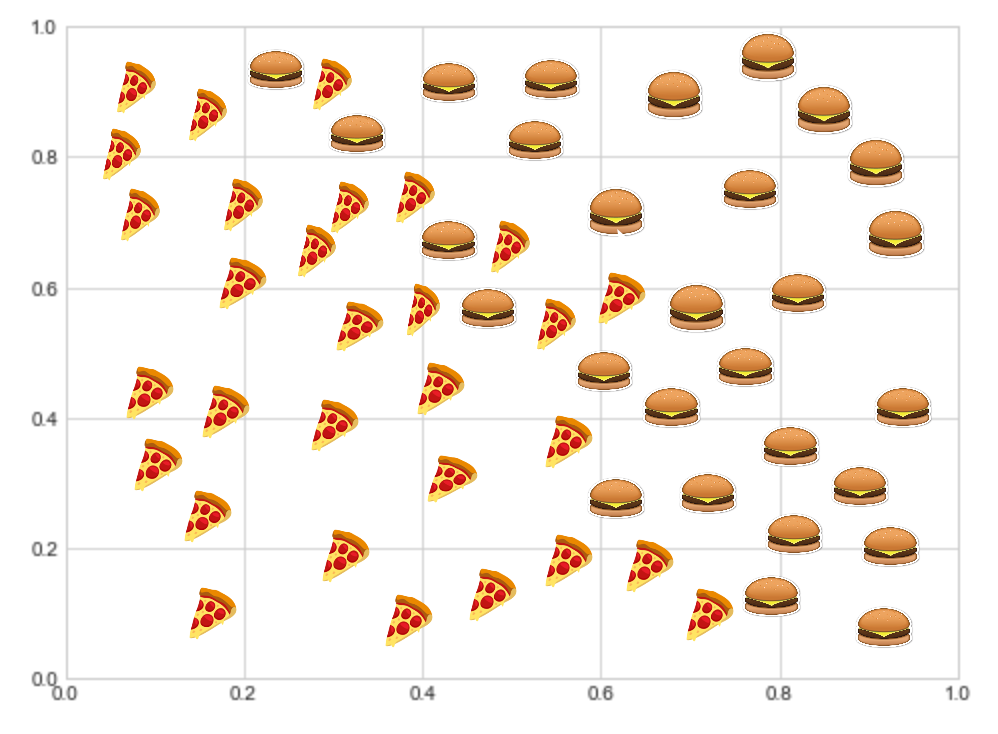
\includegraphics[scale=0.21]{class_1.png}
\end{minipage}
\hfill
\begin{minipage}[t]{0.45\textwidth}
	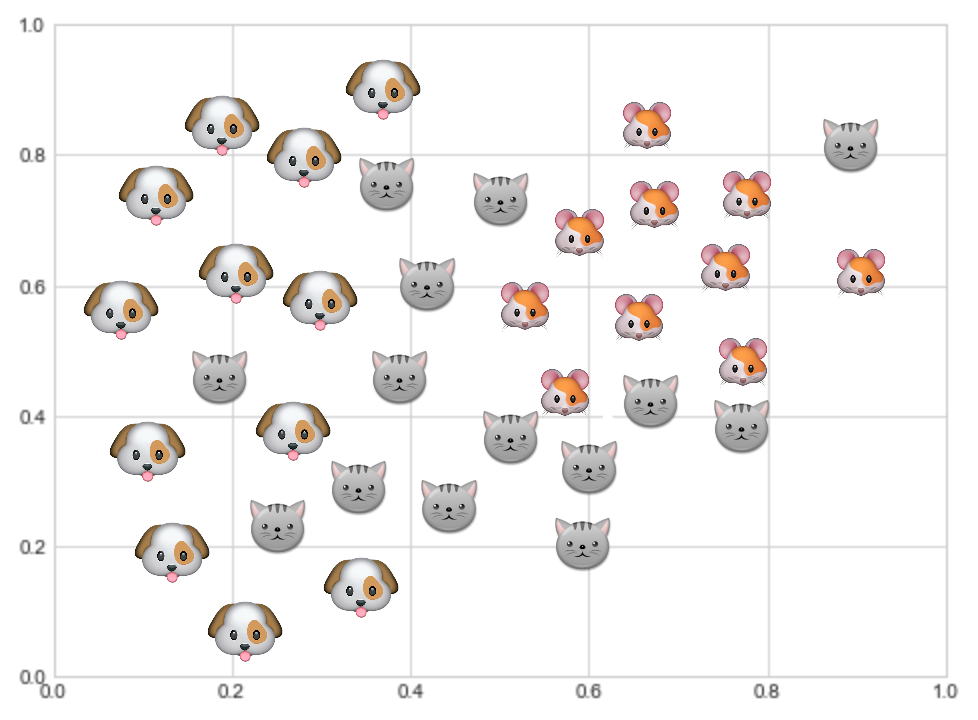
\includegraphics[scale=0.21]{class_2.png}
\end{minipage}

Почему нельзя провести между пиццей и бургерами слишком подробную и извилистую границу? В чём проблема самого правого верхнего котика? Что такое переобучение?  Как понять переобучились ли мы? 

\ifbool{answers}{
	\textbf{Решение:}
	
	Сначала обсудим бургеры и пиццу.  Первый вариант: провести между ними прямую. Тогда мы в части случаев ошибёмся и признаем некотрые бургеры пиццей, а некоторые пиццы бургерами. Второй вариант: провести извилистую разделительную линию, которая чётко разграничит бургеры и пиццу. Вопрос: какой из этих двух вариантов лучше?
	
	\begin{minipage}[t]{0.45\textwidth}
		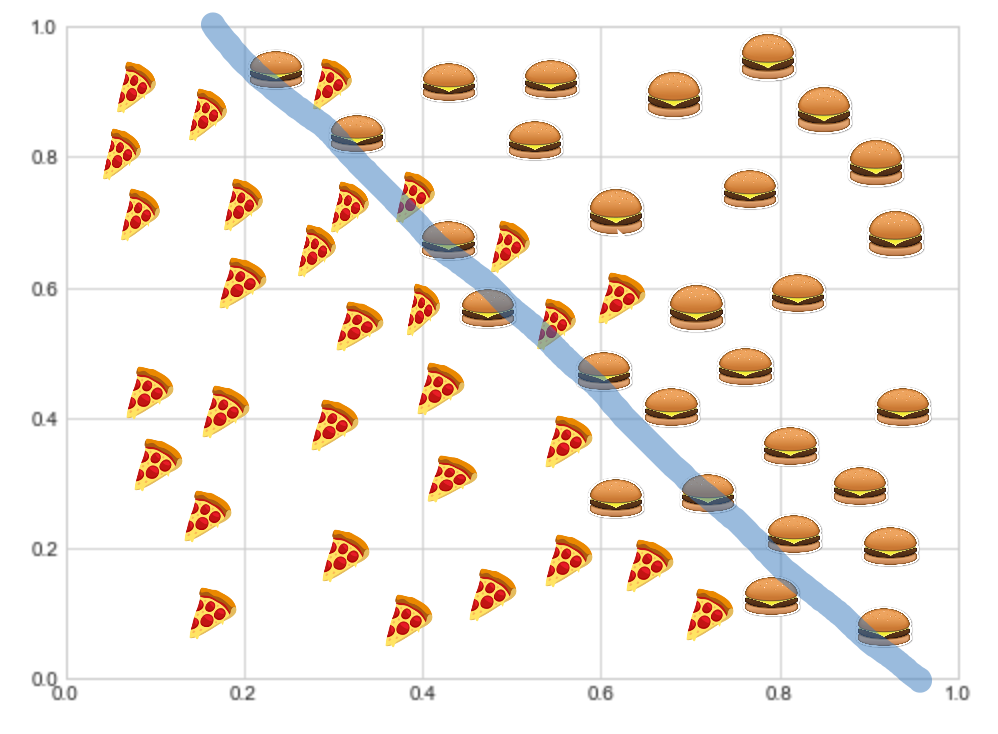
\includegraphics[scale=0.21]{class_1_res1.png}
	\end{minipage}
	\hfill
	\begin{minipage}[t]{0.45\textwidth}
		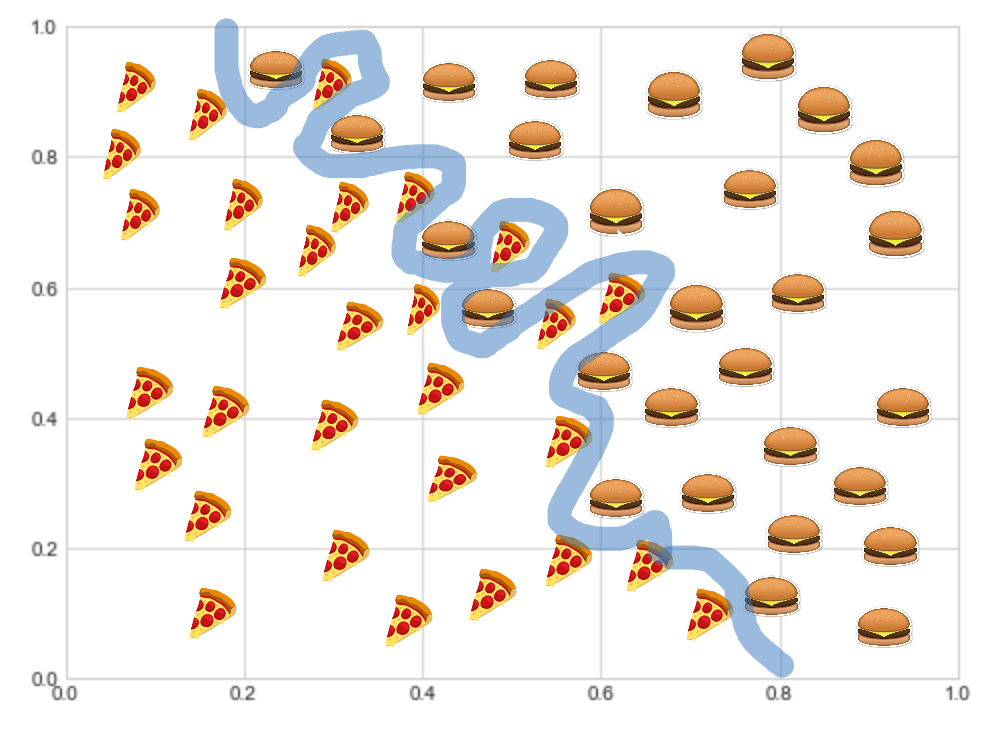
\includegraphics[scale=0.21]{class_1_res2.png}
	\end{minipage}
	
	Если у нас в выборке оказались все пиццы и бургеры мира, и других быть не может, вторая граница нам подойдёт. Мы подстроимся под все особенности нашей гениральной пицце-бургерной совокупности и будем всегда чётко и безошибочно отличать одно от другого. 
	
	\textbf{НО} в нашем распряжении обычно находится не вся генеральная совокупность, а лишь какая-то её часть. Мы в выборке видим не все возможные варианты, и хотим обучить наш классификатор обощать. Если к нам попадает новая пицуля или бургер, классификатор должен адекватно сработать на них. 
	
	Скорее всего, пиццы, проникшие на территорию бургеров, обладают какими-то аномальными особенностями, на детекцию которых затачивать классификатор нет никакого смысла. Если мы попробуем сделать это, мы влезем на территорию бургеров, и на новых объектах, которые оказались обычными бургерами, будем делать ошибки, подумав, что это аномальные пиццы. Из-за этого лучше разграничить бургеры и пиццы простой линией, которая изображена на первой картинке.
	
	\textbf{Ещё раз, ещё раз.} Если мы проведём подробную границу, мы заточим классификатор под особенности выборки, вместо того, чтобы научить его отличать пиццу от бургера в общем случае. Такие ситуации называются переобучением. И это главная головная боль людей, занимающихся машинным обучением. С переобучением у них идёт вечная борьба. 
	
	Теперь посмотрим на котиков, пёсиков и мышек. Снова мы можем провести границы между ними разными способами.
	
	\begin{minipage}[t]{0.45\textwidth}
		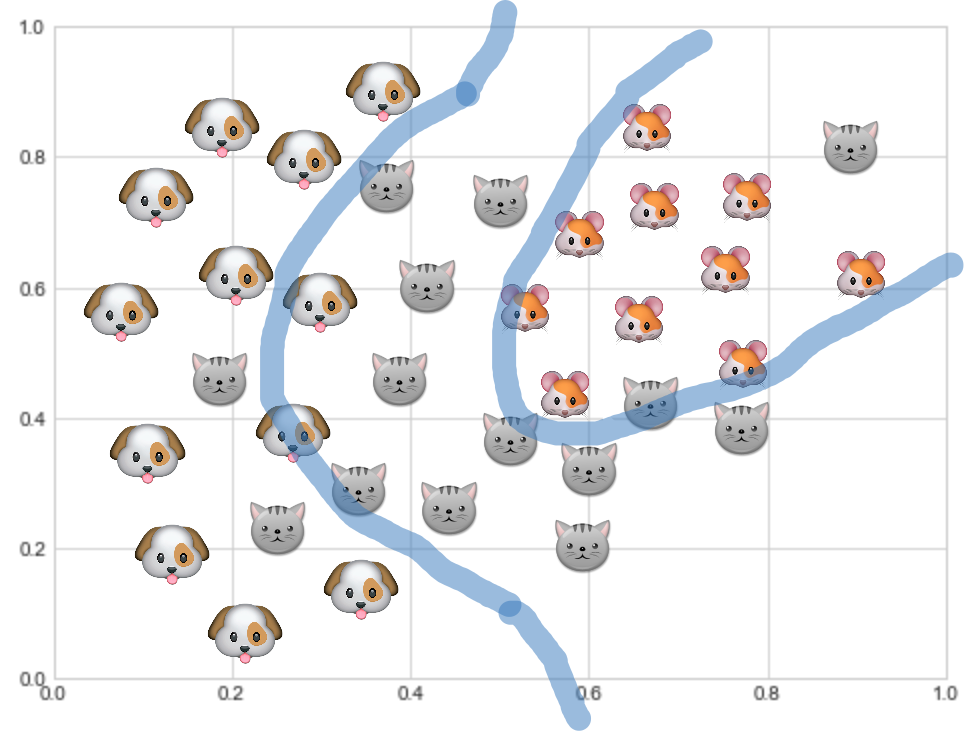
\includegraphics[scale=0.21]{class_2_res1.png}
	\end{minipage}
	\hfill
	\begin{minipage}[t]{0.45\textwidth}
		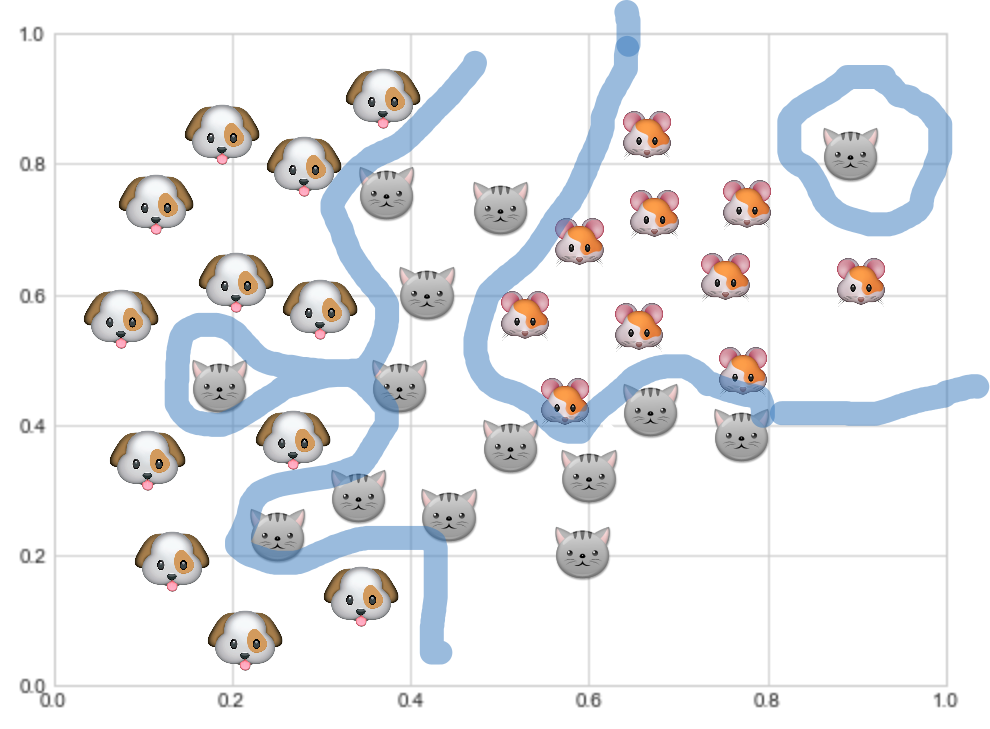
\includegraphics[scale=0.21]{class_2_res2.png}
	\end{minipage}
	
	Снова мы можем провести более-менее простую границу и иногда ошибаться. Ну знаете, есть такие собаки мелкие, похожие на кошек. Или даже на мышек. И, если мы будем специфицировать границу под этих собак, мы начнём ошибаться на котах, так как подобные аномалии встречаются редко. 
	
	Основная проблема верхнего котика в том, что он аномальный. Каким-то образом он попал на территорию мышек.  Выделять для него свою зону будет плохой идеей, так как в таком случае мы будем переобучать классификатор под конкретный выброс.
	
	\textbf{Осталось обсудить главный вопрос: как понять а не переобучились ли мы.}  Для этого обычно дробят выборку на две части: тренировочную и тестовую. На тренировочной учат алгоритм (в данном случае границу между классами), а на тестовой проверяют насколько хорошо он работает. Насколько часто алгоритм на тестовой части делает ошибку. 
	
	Если получается, что на обучающей выборке качество высокое, а на тестовой низкое --- мы переобучились и вместо того, чтобы научить модель обобщать закономерности, существующие в данных, обучили его под особенности конкретной выборки.  Если на тестовой выборке качество сравнимо с обучающей, значит мы научились извлекать какие-то реальные закономерности.
	
	Бьюсь об заклад, что для простых линий, качество на тесте для бургеров и мышек будет выше, чем для сложных.  Конечно же, простые границы оказываются хороши не всегда, но всегда имеет смысл сначала построить простую модель, а после сравнивать с ней сложные. 
}


\subsection*{Задача 2 (метрики)}

Бандерлог оценил три модели: нейросеть, случайный лес и KNN.  Он построил на тестовой выборке прогнозы и получил три матрицы ошибок: 

\begin{minipage}[t]{0.33\textwidth}
	\begin{tabular}{|c|c|c|}
		\hline
		& $y=1$  &  $ y = 0$ \\  \hline 
		$\hat y = 1$  &   $80$ &    $20$ \\      \hline 
		$\hat y = 0$ &   $20$ &     $80$ \\      \hline 
	\end{tabular}
\end{minipage}
\begin{minipage}[t]{0.33\textwidth}
	\begin{tabular}{|c|c|c|}
		\hline
		& $y=1$  &  $ y = 0$ \\  \hline 
		$\hat y = 1$  &   $48$ &    $2$ \\      \hline 
		$\hat y = 0$ &   $52$ &     $98$ \\      \hline 
	\end{tabular}
\end{minipage}
\begin{minipage}[t]{0.33\textwidth}
	\begin{tabular}{|c|c|c|}
		\hline
		& $y=1$  &  $ y = 0$ \\  \hline 
		$\hat y = 1$  &   $10$ &    $20$ \\         \hline 
		$\hat y = 0$ &   $90$ &    $10000$ \\   \hline 
	\end{tabular}
\end{minipage}

\begin{enumerate}
	\item[а)]   Найдите для всех трёх моделей долю правильных ответов. Чем плоха эта метрика? 
	\item[б)]   Найдите для всех трёх моделей точность (precision) и полноту (recall)
	\item[в)]   Предположим, что целевая переменная $y$ принимает значение $1$, если заемщик вернул кредит  и $0$, если не вернул. Вы хотите научиться прогнозировать платежеспособность клиента. Какую из первых двух моделей вы бы выбрали в таком случае? 
	\item[г)]  Предположим, что целевая переменная $y$ принимает значение $1$, если человек болен больной болезнью с болью и $0$, если он здоров. Вы хотите спрогнозировать нужно ли человеку обследование. Какую из первых двух моделей вы б выбрали в этом случае? 
\end{enumerate}

\ifbool{answers}{
	\textbf{Решение:}
	
	\begin{enumerate}
		\item[а)] 	Ежели мы совершаем ошибку, то мы делаем это спрогнозировав $\hat y = 1$ там, где реально должно быть $y = 0$ либо наоборот, прогнозируя $\hat y = 0$ там, где реально должно быть $y=1$.  В остальных случаях всё ок.  Наша классная табличка выглядит следущим образом: 
		
		\begin{center}
			\begin{tabular}{|c|c|c|}
				\hline
				& $y=1$  &  $ y = 0$ \\  \hline 
				$\hat y = 1$  &    $TP$ &     $FP$ \\      \hline 
				$\hat y = 0$ &    $FN$ &     $TN$ \\      \hline 
			\end{tabular}
		\end{center}
		
		Долю правильных ответов можно посчитать как 
		
		\[
		Accuracy = \frac{TP + TN}{TP + TN + FP + FN}.
		\]
		
		Давайте проделаем эту несложную процедуру для вердиктов всех трёх алгоритмов, описанных выше. 
		
		\begin{equation} 
		\begin{aligned}
		&Accuracy_1 = \frac{80 + 80}{80 + 80 + 20 + 20} = 0.8   \\ 
		&Accuracy_2 = \frac{48 + 98}{48 + 98 + 2 + 52} = 0.73  \\ 
		&Accuracy_3 = \frac{10 + 10000}{10 + 10000 + 20 + 90} = 0.98  \\ 
		\end{aligned}
		\end{equation} 
		
		У этой метрики есть как минимум две существенные проблемы. 
		
		Первая проблема связана с несбалансированными выборками. Именно такая ситуация наблюдается в третьей табличке. Нулевой класс заметно перетягивает на себя выборку. Выходит, что если мы просто-напросто спрогнозируем, что все объекты в выборке нулевые, мы получим табличку 
		
		\begin{center}
			\begin{tabular}{|c|c|c|}
				\hline
				& $y=1$  &  $ y = 0$ \\  \hline 
				$\hat y = 1$  &   $0$ &    $0$ \\         \hline 
				$\hat y = 0$ &   $100$ &    $10020$ \\   \hline 
			\end{tabular}
		\end{center}
		
		и $Accuracy = 0.99$. Наша модель показала более низкое качество, чем простое угадывание. Выходит, что наша модель абсолютно бесполезна. 
		
		Чтобы «бороться» с этой проблемой, используется следующий факт. Пусть $q_0$ — доля объектов самого крупного класса, тогда доля правильных ответов для разумных алгоритмов $accuracy \in [q_0,1]$, а не $[0.5, 1]$, как это можно было бы ожидать. Поэтому, если получается высокий процент правильных ответов, это может быть связано не с тем, что построен хороший классификатор, а с тем, что какого-то класса сильно больше, чем остальных.
		
		Вторая проблема с долей верных ответов состоит в том, что она никак не учитывает разные цены разных типов ошибок. Тогда как цены действительно могут быть разными.
		
		Например, представим себе линейное небо, которое бороздят вражеские самолёты. Мы стоим на земле, у нас есть пушка и снаряды. Сбивать вражеские самолёты можно руководствуясь двумя разными стратегиями: 
		
		\textbf{Путь первый:}  стрелять по всему небу, куда только можно попасть. В таком случае точность наших выстрелов будет низкой, но зато мы собьём все самолёты, то есть добьёмся высокой полноты. Такая стратегия на картинке прорисована красными лазерными выстрелами из пушки.
		
		\textbf{Путь второй:} стрелять поточнее, пореже. Тогда мы будем сбивать самолёты точно, потратим мало снарядов вхолостую, но собьём не все самолёты. Такая стратегия на картинке прорисована зелёными выстрелами из пушки. 
		
		\begin{center}
			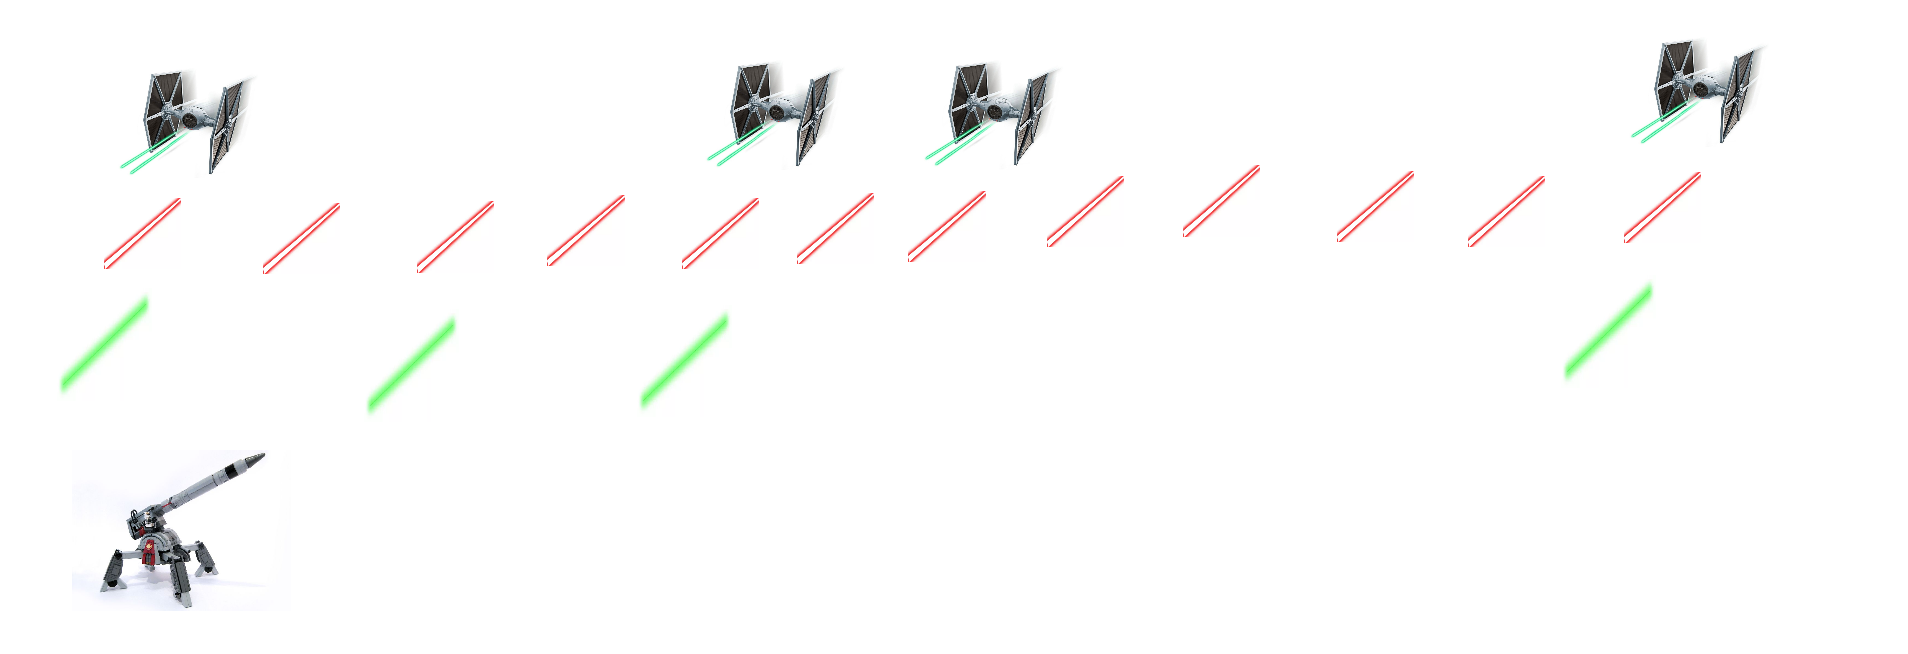
\includegraphics[width=.79\paperwidth]{fly.png}
		\end{center}
		
		
		Для разных задач бывают характерны разные стратегии. Если вернуться к нашей исходной таблице ошибок, то за точность классификатора будет отвечать первая строка
		
		\[ 
		Precision = \frac{TP}{TP + FP}.
		\]
		
		За полноту будет отвечать первы столбец
		
		\[Recall = \frac{TP}{TP + FN}.\]
		
		Посмотрим ещё один пример: если мы решаем задачу крединтого скоринга, нам нужно получить деньги назад после выдачи кредитов, иначе мы разоримся. Нам нужна модель, которая будет точно определять надёжного заёмщика. В этой ситуации для нас неважно покрыть все вражеские истребители снарядами (выдать кредиты каждому надёжному заёмщику), для нас важно сделать это точно. Поэтому основное внимание мы уделяем ошибке $FP$. 
		
		Если мы пытаемся найти больных больной болезнью с болью и отправить их делать дополнительные анализы, для нас страшнее $FN$ ошибка. Если мы отправим лишнего человека на анализы, ничего страшного с ним не произойдёт. Если мы забудем проверить больного, он умрёт. Тут лучше добиться высокой полноты, при небольшой точности. 
		
		В разных ситуациях ошибки имеют разные цены. $Accuracy$ не видит этого, поэтому на практике обычно используют $Precision$ и $Recall$. 
		
		\item[б)]  
		
		\begin{equation} 
		\begin{aligned}
		&Precision_1 =  0.8   \qquad &Recall_1 = 0.8 \\ 
		&Precision_2 = 0.96  \qquad &Recall_2 = 0.48 \\ 
		&Precision_3 = 0.33  \qquad &Recall_3 = 0.1  \\
		\end{aligned}
		\end{equation} 
		
		Вторая модель является очень точной, но в ущерб полноте. Третья модель очень плохая. Эти две метрики, в отличие от $Accuracy$, позволили заметить этот факт. 
		
		\item[в)] При использовании первой модели кредит будет выдан 100 клиентам, 80 из которых его вернут. Во второй модели, более консервативной, кредит был выдан только 50 клиентам, причем вернули его в 48 случаях. 
		
		Выше мы обсудили, что бизнес-специфика задачи диктует нам необходимость взять модель, где побольше точность.
		
		\item[г)]  Выше мы обсудили, что нам нужна модель, где побольше полнота.
	\end{enumerate}
}


\subsection*{Задача 3 (ещё немного метрик)}

Бандерлог из Лога\footnote{деревня в Кадуйском районе Вологодской области} ведёт блог, любит считать логарифмы и оценивать модели. С помощью нового алгоритма Бандерлог решил задачу классификации по трём наблюдениям и получил $b_i = \hat P(y_i = 1|x_i)$.

\begin{center}
	\begin{tabular}{c|c}
		$y_i$ & $b_i$ \\
		\hline
		$1$  & $0.7$ \\
		$0$ & $0.2$ \\
		$0$ & $0.3$ \\
		$1$ & $0.25$ \\
	\end{tabular}
\end{center}

\begin{enumerate}
	\item[a)] Найдите ROC AUC.
	\item[б)] Постройте ROC-кривую.
	\item[в)] Постройте PR-кривую (кривая точность-полнота).
	\item[г)] Найдите площадь под PR-кривой.
	\item[д)] Как по-английски будет «бревно»?
\end{enumerate}

\ifbool{answers}{
	\textbf{Решение:}
	
	\begin{enumerate}	
		\item[а)]  В предыдущей задаче мы немного обсудили метрики классификации. Когда мы на практике оцениваем модель, она выплёвывает в нас не принадлежность объекта к классу в явном виде, а вероятности того, что наши объекты --- единички. 
		
		Например, давайте думать в терминах оттока клиентов. Пусть наш сервис привлёк каких-то ребят в постоянные пользователи. Если они начнут унывать, им захочется свалить. Это называется оттоком. Давайте предположим, что модель выдаёт нам вероятность того, что человек решил приуныть. Если мы сможем понимать кто собрался приуныть, будем одаривать их ништяками и тогда они будут оставаться нашими клиентами. 
		
		Как понять, кто собирается приуныть, если модель выплёвывает на нас вероятности? Давайте выберем порог и будем считать, что все, у кого вероятность уныния $\ge 0.5$ --- отностяся к классу $1$. Есть вероятность, что они решат свалить. Их и будем одаривать ништяками. В нем случае получатся прогнозы: $1,0,0,0$. Если взять порог $0.3$, получим прогнозы $1,0,1,0$. 
		
		Как выбрать порог, кого одаривать ништяками. Если у нас большой бюджет, можно попробовать поставить низкий порог, чтобы добиться большой полноты. Если маленький бюджет, то давайте поставим порог так, чтобы борьба с унынием была поточнее. Выбор порога зависит от специфики бизнеса и от того, что от нас хотят. 
		
		Видно, что точность и полнота зависят от выбора порога. А хотелось бы, чтобы та метрика, по которой мы выбираем модель, от порога не зависила. Так рождаются идеи о метриках $roc_auc$ и $pr_auc$. 
		
		Представим себе два объекта: приунывший и нормальный. Представим себе, что модель предсказала нам вероятность уныния для первого объекта $b_1$ и для второго $b_2$.
		
		\begin{equation} 
		\begin{aligned}
		&y = 1   \qquad &\hat P(y = 1) = b_1\\ 
		&y = 0  \qquad & \hat P(y = 1) = b_2\\ 
		\end{aligned}
		\end{equation} 
		
		Если у нас хорошая модель, то явно $b_1 > b_2$. Иначе модель всё путает и говорит, что неунывающие приуныли. Давайте посмотрим как часто на нашей выборке такая путаница происходит и рассмотрим все возможные пары нулей и единичек. Всего будет четыре пары. 
		
		\begin{equation} 
		\begin{aligned}
		& 0.7 > 0.2 \qquad & ok \\
		& 0.7 > 0.3 \qquad & ok \\
		& 0.25 > 0.2 \qquad & ok \\ 
		& 0.25 < 0.3 \qquad & not \mbox{ } ok \\
		\end{aligned}
		\end{equation} 
		
		Видим, что модель ошиблась в упорядочивании один раз. $roc_auc$ --- это доля пар, где модель оказалась права. В нашем случае это $0.75$. $roc_auc$ принимает значения от $0.5$ до $1$, если её значения близки к $0.5$, наш алгоритм ничем не лучше монетки, потому что он упорядочивает пары из унывших и нормальных абы как. 
		
		Такая метрика позволяет не привязываться к конкретному значению порога и видеть насколько классно у модели выходит упорядочивать пары объектов. 
		
		\item[б)]  Величина, которую мы посчитали выше является площадью под roc-кривой (roc = receiver operating characteristic, иногда говорят «кривая ошибок»), с помощью которой часто визуализируют качество работы алгоритма.  Когда говорять про roc-auc имется в виду area under the curve. 
		
		Чтобы нарисовать ROC-кривую, надо взять единичный квадрат на координатной плоскости, разбить его на m равных частей горизонтальными линиями и на $n$ – вертикальными, где $m$ – число $1$ среди правильных меток теста (в нашем примере $m=2$), $n$ – число нулей ($n=2$). В результате квадрат разбивается сеткой на $m \times n$ блоков.
		
		Отсортируем нашу табличку по значению вероятности, которую предсказала модель. 
		
		\begin{center}
			\begin{tabular}{c|c}
				$y_i$ & $b_i$ \\
				\hline
				$1$  & $0.7$ \\
				$0$ & $0.3$ \\
				$1$ & $0.25$ \\
				$0$ & $0.2$ \\
			\end{tabular}
		\end{center}
		
		Теперь будем просматривать строки сверху вниз и прорисовывать на сетке линии, переходя их одного узла в другой. Стартуем из точки $(0, 0)$. Если значение метки класса в просматриваемой строке $1$, то делаем шаг вверх; если $0$, то делаем шаг вправо. Ясно, что в итоге мы попадём в точку $(1, 1)$, т.к. сделаем в сумме $m$ шагов вверх и $n$ шагов вправо.
		
		
		\begin{center}
			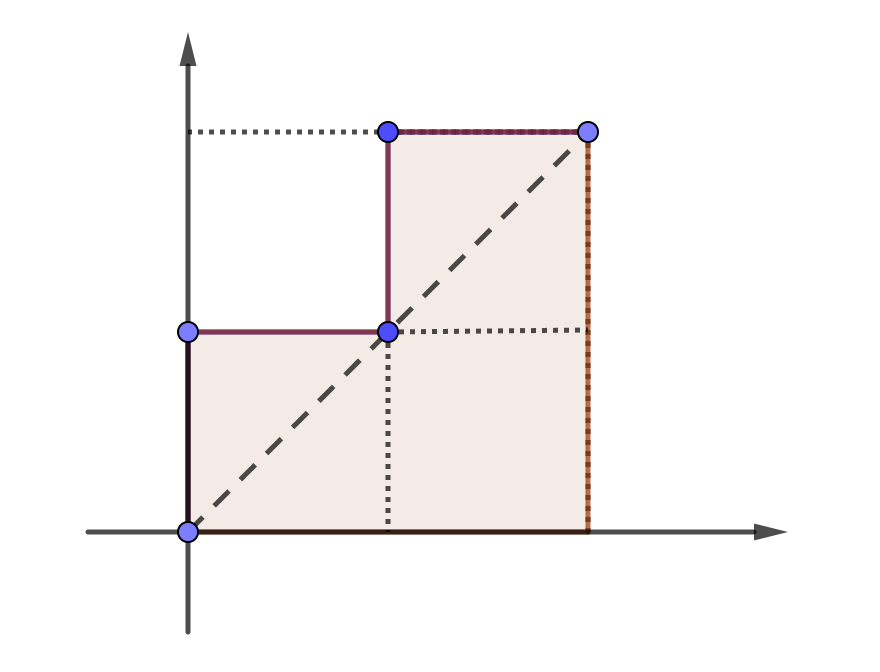
\includegraphics[width=.4\paperwidth]{roc_auc.png}
		\end{center}
		
		Сетка разбила квадрат на  $m \times n$ блоков. Ровно столько же пар вида (объект класса $1$, объект класса $0$), составленных из объектов тестовой выборки. Каждый закрашенный блок соответствует паре (объект класса $1$, объект класса $0$), для которой наш алгоритм правильно предсказал порядок (объект класса $1$ получил оценку выше, чем объект класса $0$), незакрашенный блок – паре, на которой ошибся.
		
		\item[в)] Давайте по оси $x$ откладывать полноту, а по оси $y$ точность. Давайте по очереди перебирать разные пороги и считать для них точность и полноту. Нанесём на картинку все полученные точки и соединим их. Это и будет $PR$-кривая. 
		
		Например, если мы возьмём порог $ \ge 0.2$, тогда все объекты будут принадлежать к классу $1$ точность составит $0.5$, а полнота $1$.  Если мы возьмём порог $\ge 0.25$, тогда один объект будет нулевым, а остальные три единичными.  Точность составит $0.66$, а полнота $1$.  По аналогии получим точность и полноту при порогах $\ge 0.3$ и $\ge 0.7$. 
		
		\begin{center}
			\begin{tabular}{c|c|c}
				порог &точность  & полнота\\
				\hline
				$0.2$ & $0.5$ & $1$ \\
				$0.25$ & $0.66$ & $1$ \\
				$0.3$ & $0.5$ & $0.5$ \\
				$0.7$ & $1$ & $0.5$ \\
				$0.8$ & $0$ & $0$ \\
			\end{tabular}
		\end{center}
		
		Строим кривую! 
		
		\begin{center}
			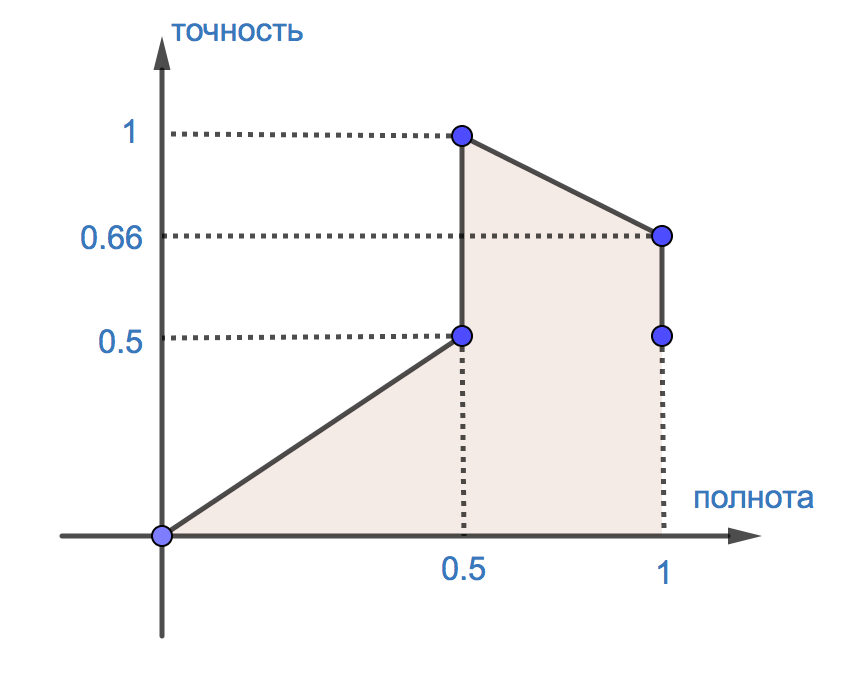
\includegraphics[width=.4\paperwidth]{pr_rc.png}
		\end{center}
		
		PR- кривая всегда начинается из точки $(0,0)$ и заканчивается в точке $(1,r)$, где $r$ --- это доля объектов первого класса в выборке. 
		
		В случае идеального классификатора, то есть если существует такой порог, что и точность, и полнота равны $100\%$, кривая будет проходить через точку $(1, 1)$. Таким образом, чем ближе кривая пройдет к этой точке, тем лучше оценки. Площадь под этой кривой может быть хорошей мерой качества оценок принадлежности к классу $1$. Такая метрика называется pr-auc, или площадь под PR-кривой.
		
		
		\item[г)] Посчитав площадь под кривой получим pr-auc.  Будем делать это, считая площади треугольников и прямоугольников. 
		
		\[
		1 - 0.5^2 - 0.5^2 \cdot 0.5 - 0.33 \cdot 0.5 \cdot 0.5 = 0.542
		\]
		
		Эта метрика подобно roc-auc не зависит от выбора порога и отражает способность модели правильно упорядочивать пары, но немножечко в другом плане.  Эта метрика строится в осях точность и полнота. Из-за этого она чувствительна к дисбалансу в классах. 
		
		Можно посмотреть на метрику roc-auc немного иначе.  Ввести две дроби
		
		\[TPR = \frac{TP}{TP +FN} \qquad FPR = \frac{FP}{FP +TN}, \]
		
		перебирать порог и в осях, соответсвующих $TPR$ и $FPR$ отмечать точки. В итоге получится ровно такая же кривая как у нас. Именно такое определение вы встретите в большинстве курсов по ML. Но любой нормальный человек сразу же забывает что означают эти $FPRFRTPRPR$, поэтому мы так делать не будем. 
		
		Единственный профит от такого определения в том, что сразу же видно, что roc-auc устройчив к дисбалансу в классах. 
		
		\item[д)]  log 
		
	\end{enumerate}
}



\subsection*{Задача 4 (KNN, кросс-валидация)}

На плоскости расположены колонии рыжих и чёрных муравьёв. Рыжих колоний три и они имеют координаты $(-1, -1)$, $(1, 1)$ и $(3, 3)$. Чёрных колоний тоже три и они имеют координаты $(2, 2)$, $(4, 4)$ и $(6, 6)$.

\begin{enumerate}
	\item[а)] Поделите плоскость на «зоны влияния» рыжих и чёрных используя метод одного ближайшего соседа.
	\item[б)] Поделите плоскость на «зоны влияния» рыжих и чёрных используя метод трёх ближайших соседей.
	\item[в)] С помощью кросс-валидации с выкидыванием отдельных наблюдений выберите оптимальное число соседей $k$ перебрав $k \in \{1, 3, 5\}$. Целевой функцией является количество несовпадающих прогнозов.
\end{enumerate}


\ifbool{answers}{
	\textbf{Решение:}
	
	\begin{enumerate}
		\item[а)]  Будем ради удобства измерять расстояние между муравейниками в метрах. Давайте отметимна плоскости несколько рандомных точек и посмотрим к чьей зоне влияния они относятся. 
		
		\begin{center}
			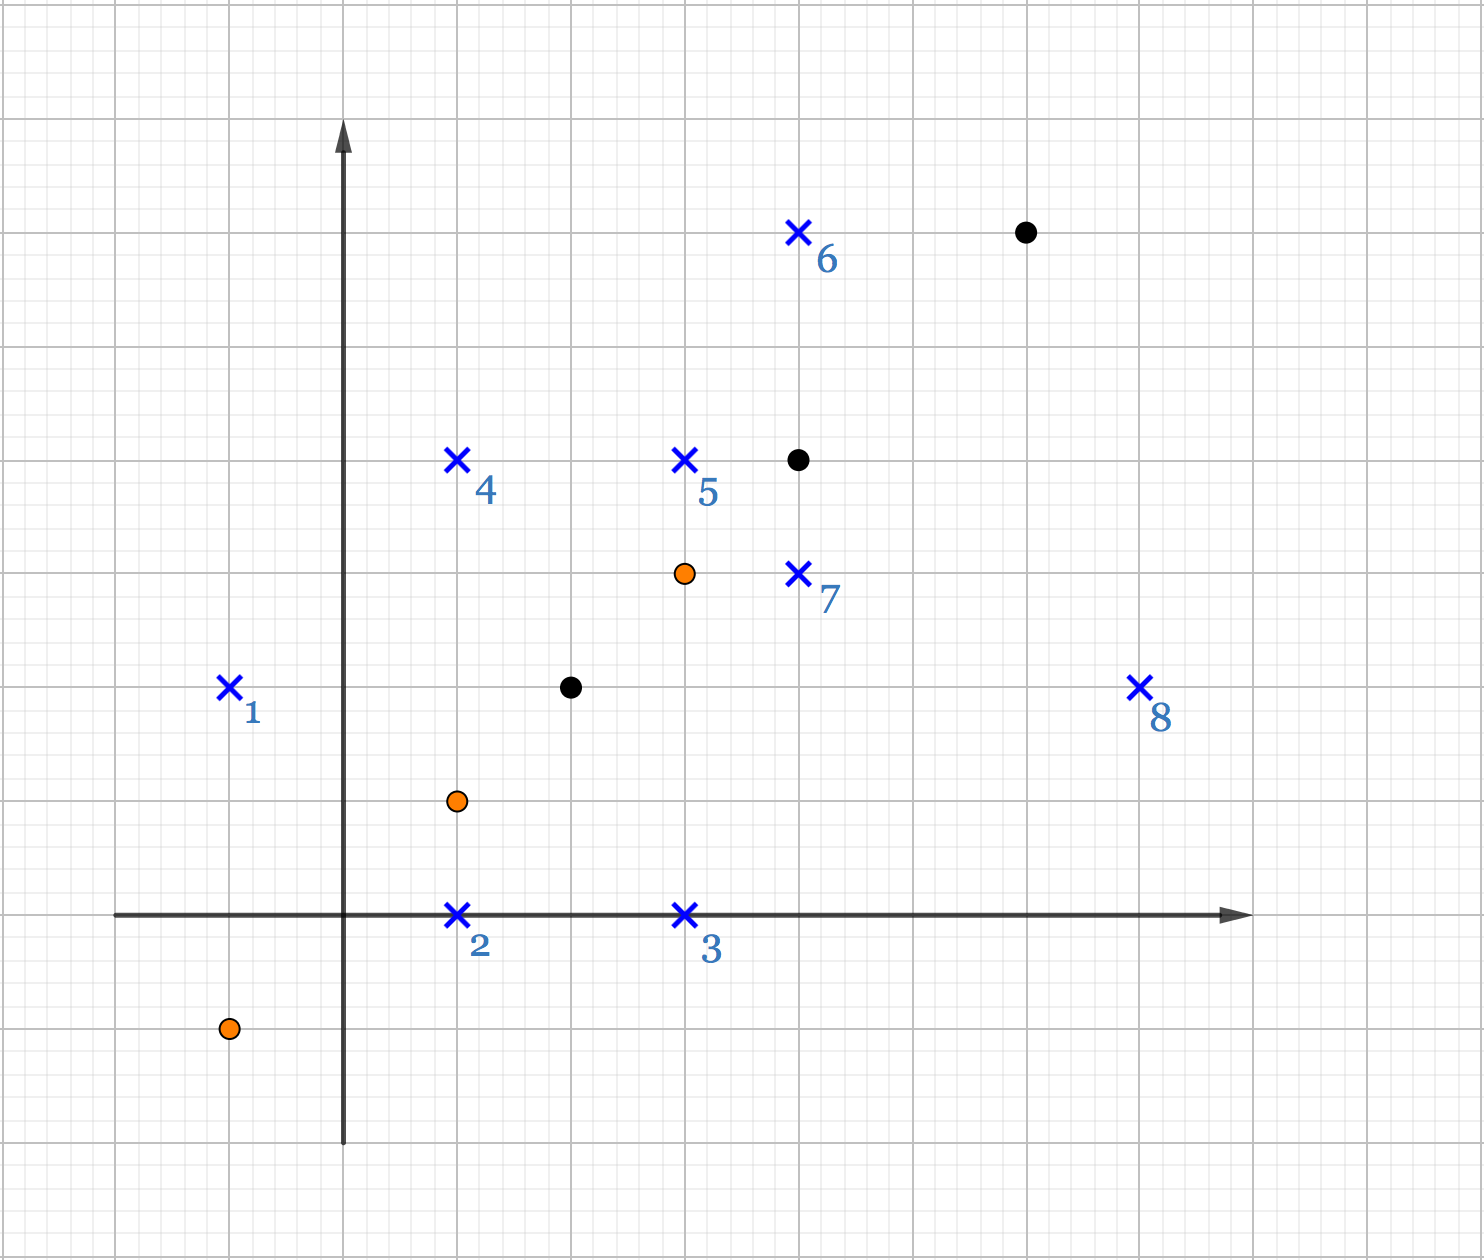
\includegraphics[scale=0.18]{2knn_1.png}
		\end{center} 
		
		Точка номер один явно будет в зоне влияния рыжих муравьёв. До ближайшего рыжего муравейника нужно пройти $\sqrt{5}$ метров, до ближайшего чёрного $3$ метра.  Точка два тоже рыжая. 
		
		По аналогии точки восемь и шесть оказыватся чёрными.  С оставшимися точками возникают проблемы. Например, от точки номер пять одинаковое расстояние как до чёрного, так и до рыжего муравейников. Она является спорной. Судя по всему, именно через неё пройдёт граница. Давайте попробуем нащупать побольше подобных пограничных точек. 
		
		Если точка принадлежит рыжим муравьям, будем помечать её рыжим крестом. Если чёрным, то чёрным. Если это спорная точка, то синим. 
		
		\begin{center}
			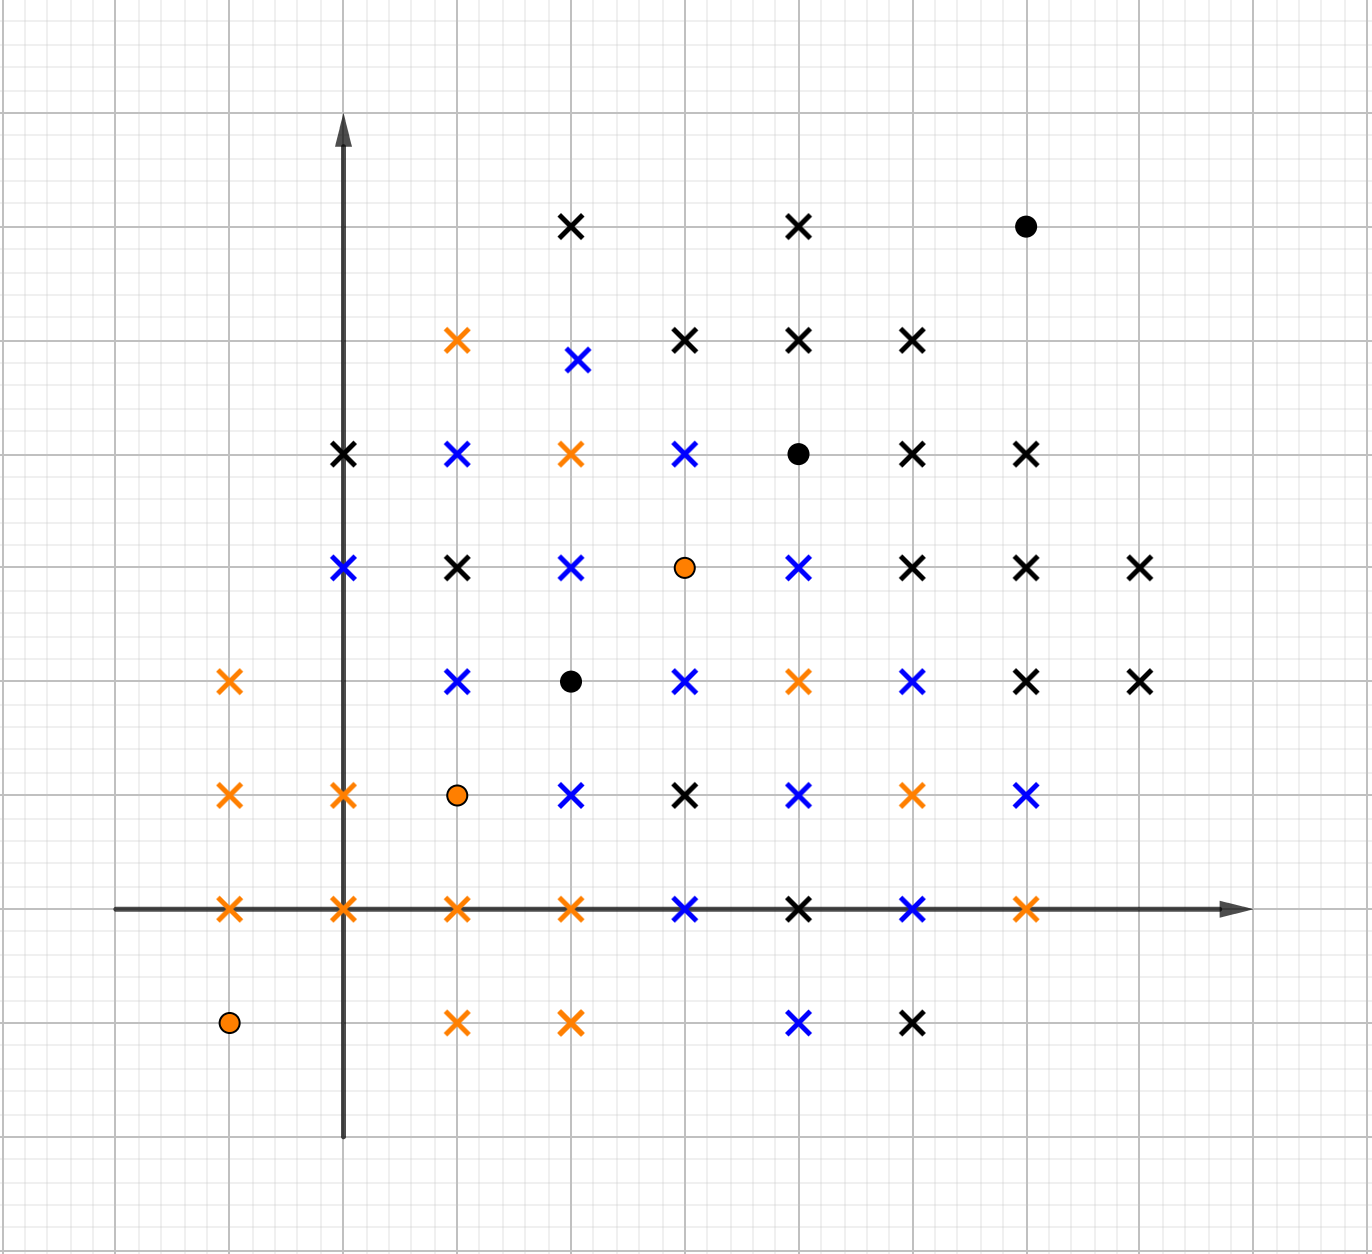
\includegraphics[scale=0.18]{2knn_2.png}
		\end{center} 
		
		Кажется, что мы нащупали границы, вдоль которых находятся спорные территории. Осталось только прочертить их.	
		
		\begin{center}
			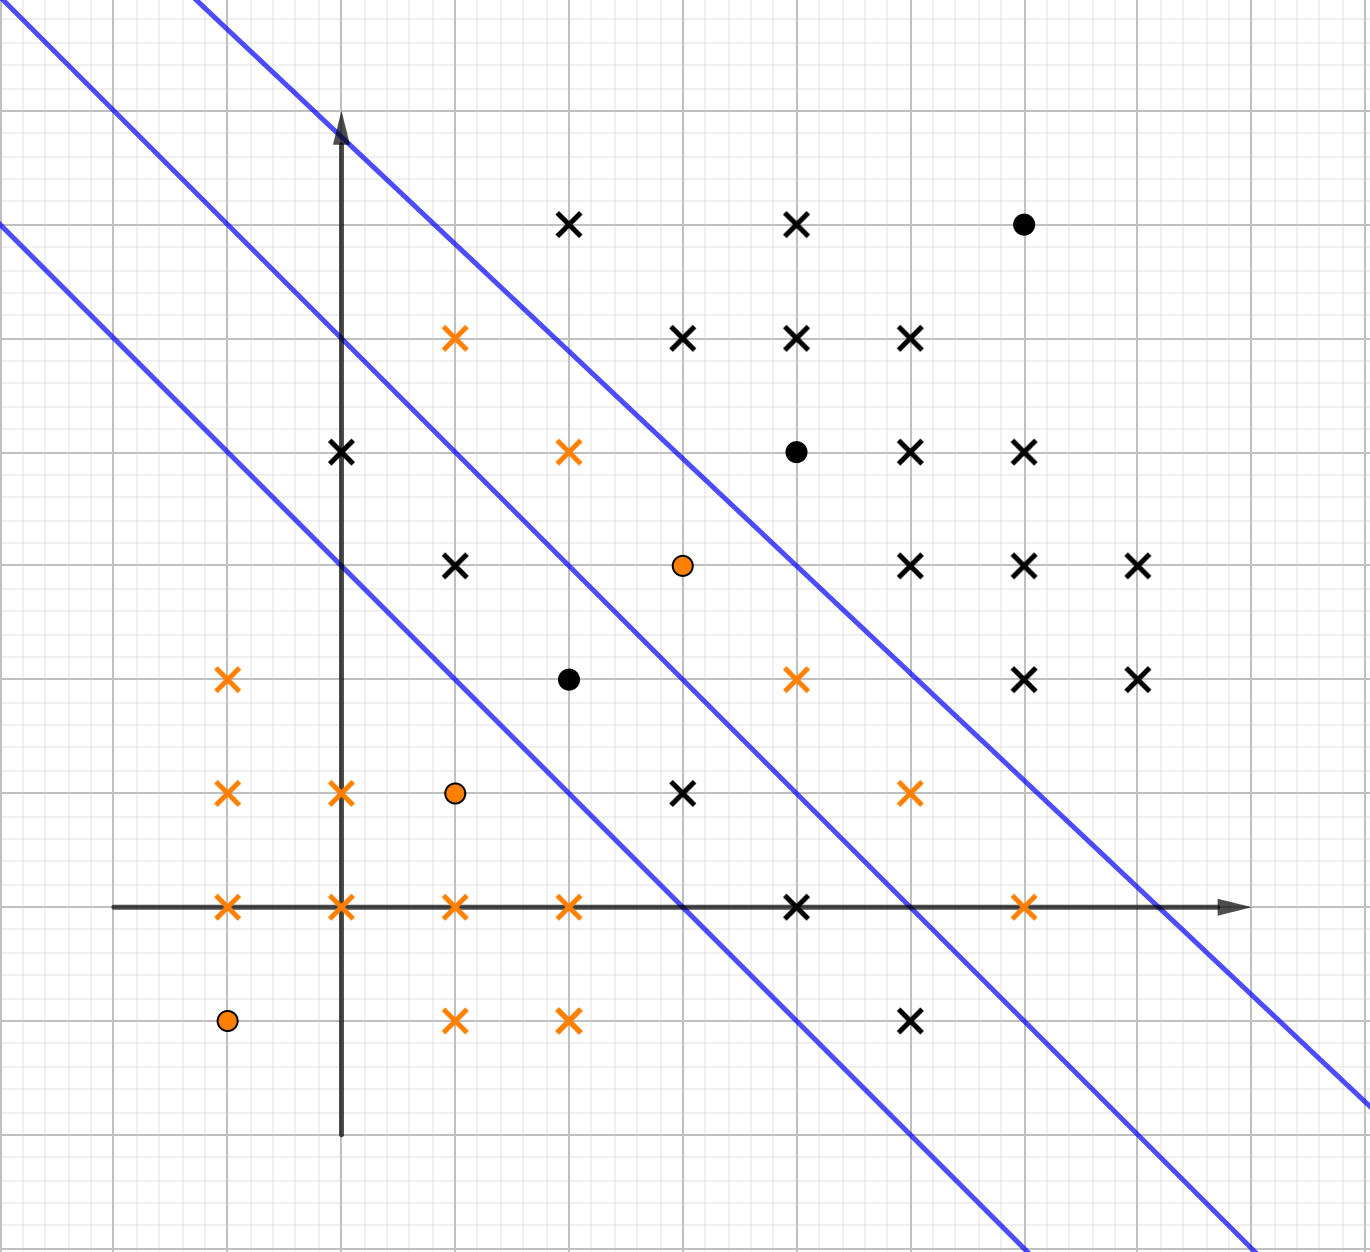
\includegraphics[scale=0.18]{2knn_3.png}
		\end{center} 
		
		\item[б)]  Теперь попробуем поделить плоскость на зоны влияния, используя метод трёх ближайших соседей. Посмотрим на самую первую картинку, где мы нанесли на плоскость рандомные точки, и попробуем порассуждать в чьей зоне влияния оказывается какая точка. 
		
		Для первой точки две из трёх ближайших --- рыжие. Она находится в рыжей зоне влияния. По аналогии происзодит со второй и третьей точками.  Пятая, шестая, седьмая и восьмая точки оказываются в зоне влияния чёрных муравьёв и окрашиваются в чёрные цвета. Проблемы возникают только с четвёртой точкой. Ближайшие к ней две точки --- рыжая и чёрная. Решение надо принимать по третьему ближайшему соседу. Третью ближайшую точку найти не удаётся, так как рыжая и чёрная точка находятся от неё н одинаковых расстояниях. Выходит, что мы оказались на границе.
		
		\begin{center}
			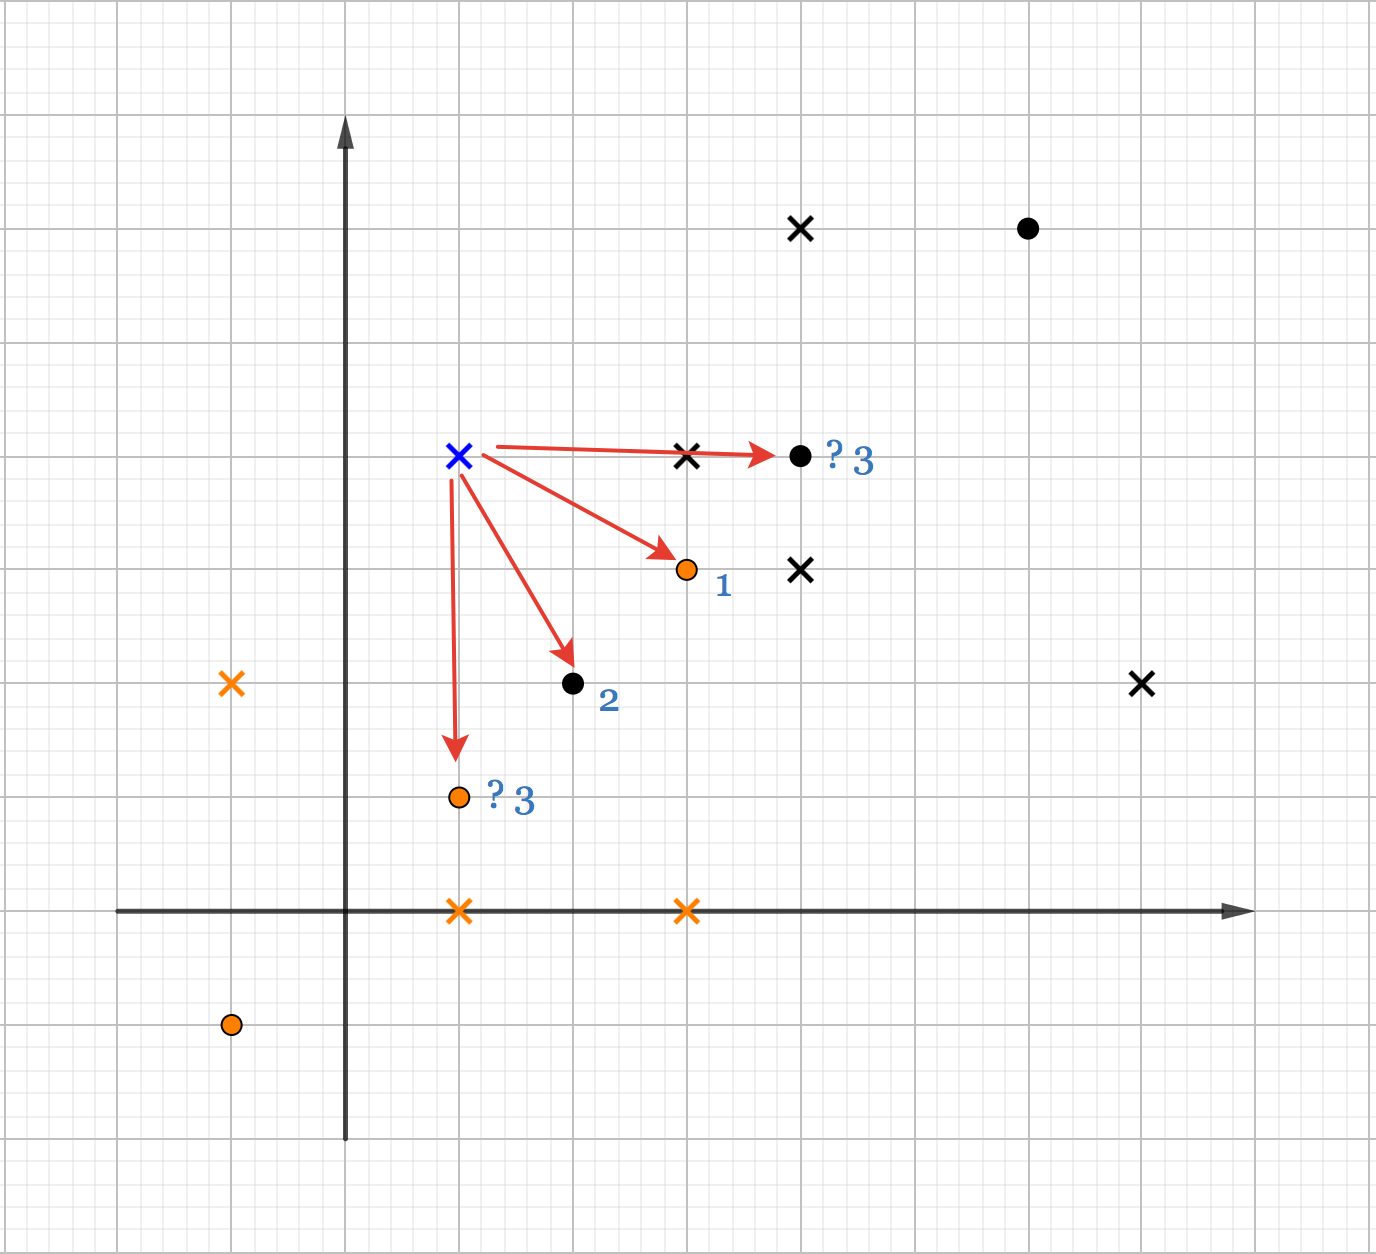
\includegraphics[scale=0.18]{2knn_4.png}
		\end{center} 
		
		Попробуем нащупать ешё пограничных точек и провести пограничную линию. 
		
		\begin{center}
			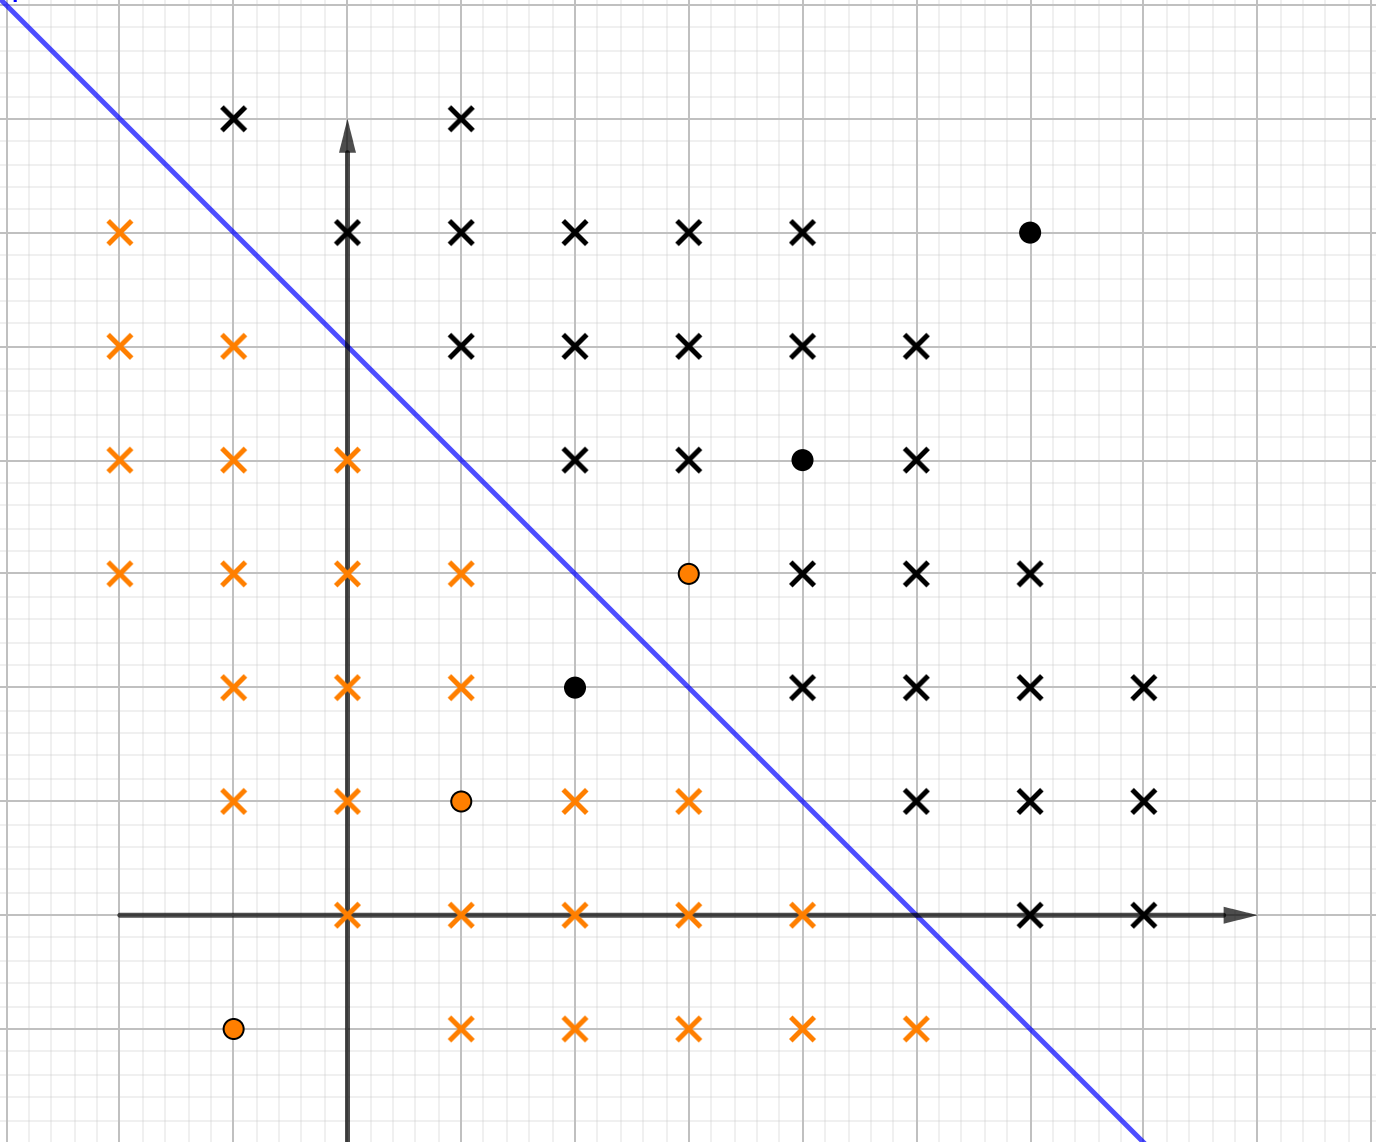
\includegraphics[scale=0.18]{2knn_5.png}
		\end{center} 	
		
		И это граница? У нас же есть ошибки!  Да, есть. Но давайте вспомним мораль, которую мы извлекли из первого упражнения: слишком детализированная граница между классами приводит к переобучению. 
		
		Порассуждаем в терминах джунглей. Есть поле, на нём селятся муравьи. Логично ли с их стороны селиться полосками? Конечно же нет. Намного логичнее было бы, что по историческим причинам на одной стороне поля живут рыжие муравьи, на второй чёрные. У нас в выборке оказалось несколько примеров муравейников. И по ним мы попытались нащупать границу для зон влияния. На границе вполне может происходить такое, что муравьи проникают на территорию друг-друга. 
		
		Проводя излишние полосы, мы переходим от выуживания реальных закономерностей, существующих в джунглях, к излишнему фрагментированию обучающей выборки, то есть переобучаемся под её особенности.  
		
		
		\item[в)]  Давайте убедимся в том, что алгоритм трёх ближайших соседей, проводящий одни разграничительную линию между муравьями, работает лучше, чем алгоритм одного ближайшего соседа. Для этого воспользуемся стратегией кросс-валидации. 
		
		Кросс-валидация состоит в следующем: давайте будем закрывать по очереди разные части выборки ладошкой. На оставшейся выборке будем обучать модель, а на скрытой проверять её качество. Будем делать так много раз и посмотрим на итоговое качество. 
		
		
		\begin{minipage}[t]{0.45\textwidth}
			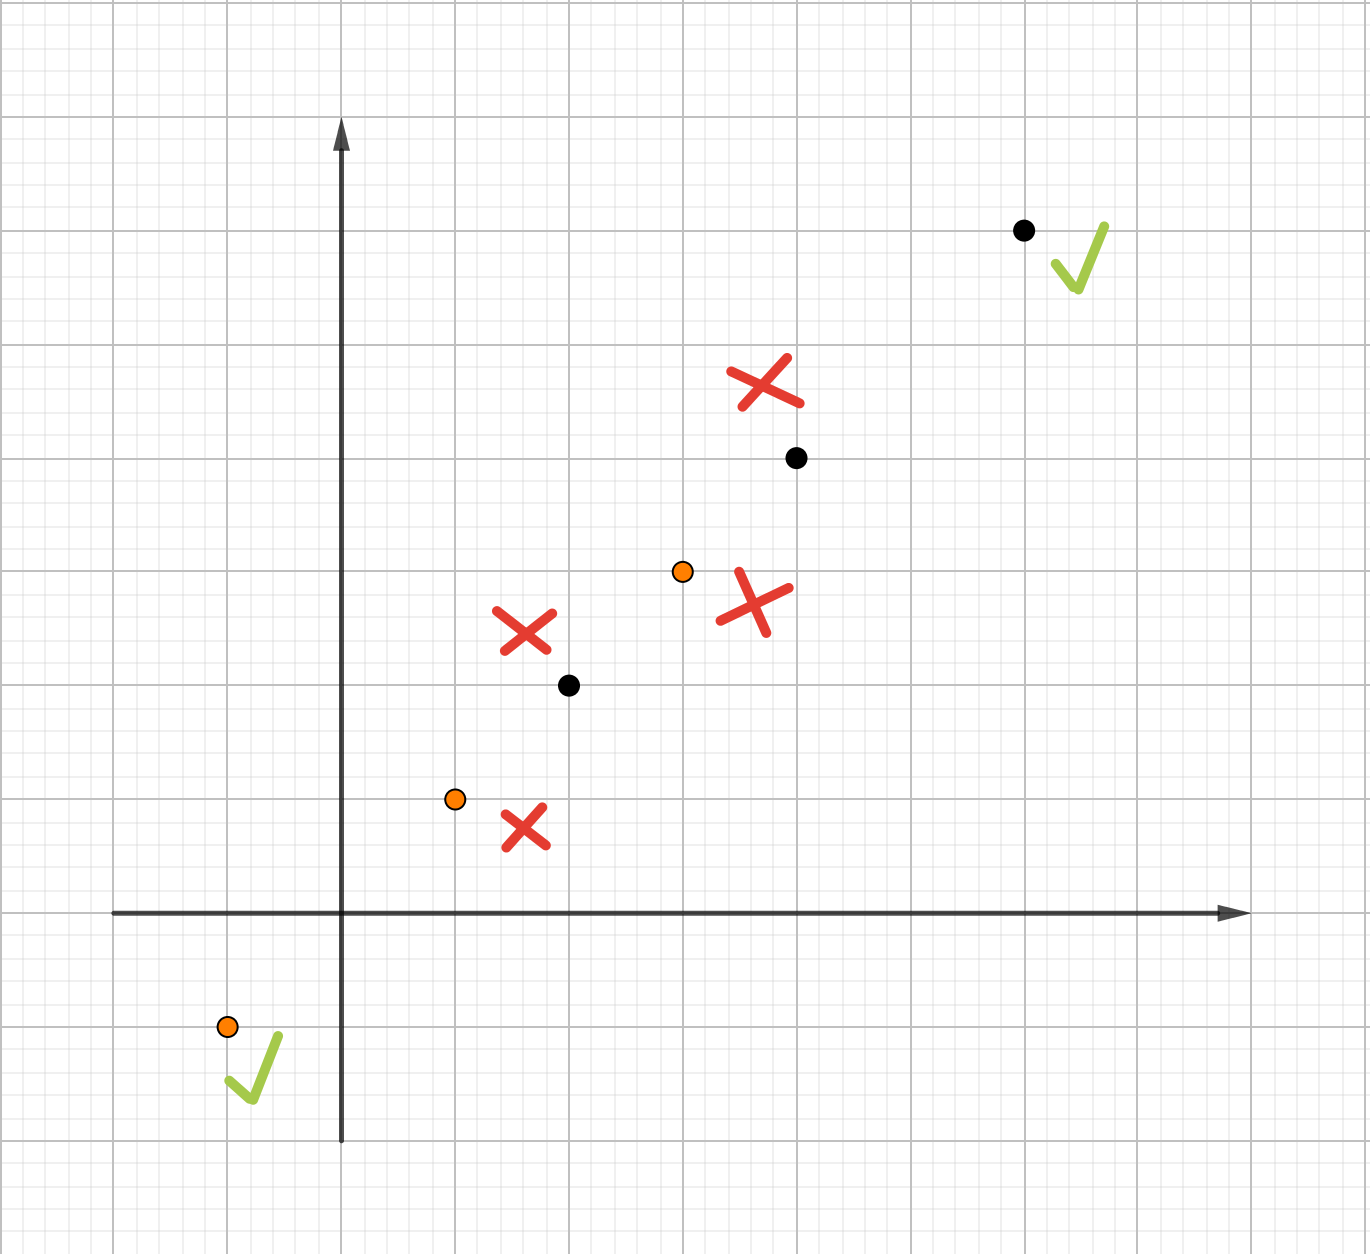
\includegraphics[scale=0.15]{2knn_6.png}
		\end{minipage}
		\hfill
		\begin{minipage}[t]{0.45\textwidth}
			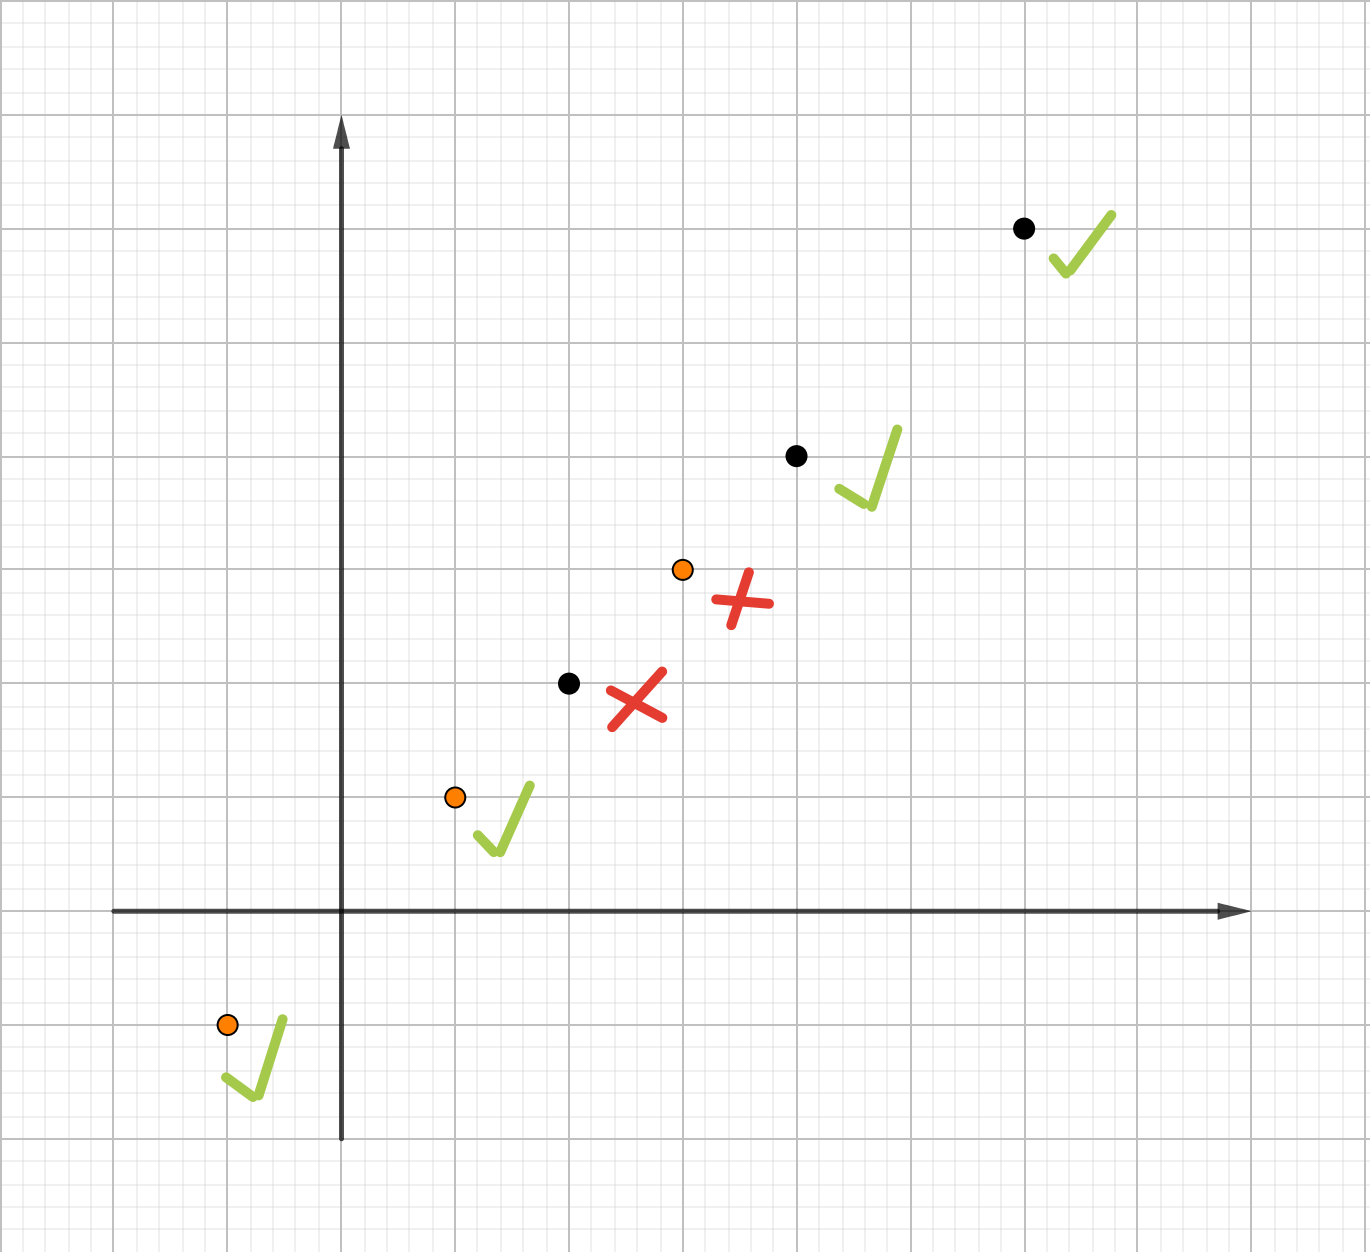
\includegraphics[scale=0.15]{2knn_7.png}
		\end{minipage}
		
		Закрываем ладошкой самую нижнюю точку. По оставшимся четырём расчерчиваем границы. Мы по методу одного ближайшего соседа относим эту точку к рыжим муравьям. Это оказывается правильным решением. Угадали.
		
		Закроем ладошкой вторую снизу точку. Расчертим границы. Она окажется ближе всего к чёрным муравьям. Но на самом деле она рыжая. Ошибка... Также проделаем с остальными точками. В итоге получится, что мы совершаем целых $4$ ошибки. По аналогии сделаем с методом трёх ближайших соседей и получим всего лишь $2$ ошибки. 
		
		Чувствуете? Мы ошибаемся из-за излишней детализации, которую нам навязывает метод одного ближайшего соседа. Кросс-валидация позволяет это отследить. А что, если взять $5$ ближайших соседей? Тогда мы ошибёмся абсолютно в каждой точке.
		
		На самом деле $k$ это гиперпараметр метода ближайших соседей. Мы можем подобрать его оптимальным образом с помощью кросс-валидации. В данном примере оптимально будет выбрать $k=3$.  
	\end{enumerate}
}



\subsection*{Задача 5 (древо для классификации)}

Машка пять дней подряд гадала на ромашке, а затем выкладывала очередную фотку «Машка с ромашкой» в инстаграмчик. Результат гадания — переменная $y_i$, количество лайков у фотки — переменная $x_i$. Постройте классификационное дерево для прогнозирования $y_i$ с помощью $x_i$ на обучающей выборке:

\begin{center}
	\begin{tabular}{cc}
		$y_i$ & $x_i$ \\
		\hline
		плюнет & $10$ \\
		поцелует & $11$ \\
		поцелует & $12$ \\
		к сердцу прижмёт & $13$ \\
		к сердцу прижмёт & $14$ \\
	\end{tabular}
\end{center}

Дерево строится до идеальной классификации. Критерий деления узла на два — минимизация числа допущенных ошибок\footnote{На самом деле на практике так не делают. Обычно для разбиения узла при строительстве классификационных деревьев используют энтропию. О том, что это такое, можно погуглить.}.  Правило прогнозирования в каждой вершине: в качестве прогноза выдаем тот класс, представителей которого в вершине больше.  Предположим, что под фоткой стоит 15 лайков, каков будет результат гадания? 


\ifbool{answers}{
	\textbf{Решение:}
	
	Мы должны обучить дерево, которое будет по переменной $x$, число лайков от парня, прогнозировать переменную $y$, состояние отношений Маши.  Обычно деревья учат по-жадному. Будем смотреть, какое разбиение по переменной $x$ сильнее всего уменьшает ошибку, и выбирать его. 
	
	Ошибку мы договорились считать как долю неверных ответов. Обычно на практике при разбиении вершины на две используют не такой критерий, но мы для простоты используем его. 
	
	При делении вершины на две между $10$ и $11$ лайкаи, слева у нас окажется плюнет. Именно его мы и будем там прогнозировать. Справа окажется два поцелует и два к сердцу прижмёт. Надо спрогнозировать в этой вершине класс, представителей которого тут большинство, чтобы сделать поменьше ошибок. Так как у нас оба класса представлены в одинаковом объёме, неважно что мы спрогнозируем. В любом случае получим две ошибки. 
	
	При дроблении вершины на две между $11$ и $12$ лайками, слева оказывается плюнет и поцелует. Одна ошибка. Справа оказывается два к сердцу прижмёт и одно поцелует. Спрогнозируем к сердцу прижмёт, так как их большинство, и получи одну ошибку. В сумме у нас две ошибки. 
	
	
	\begin{center}
		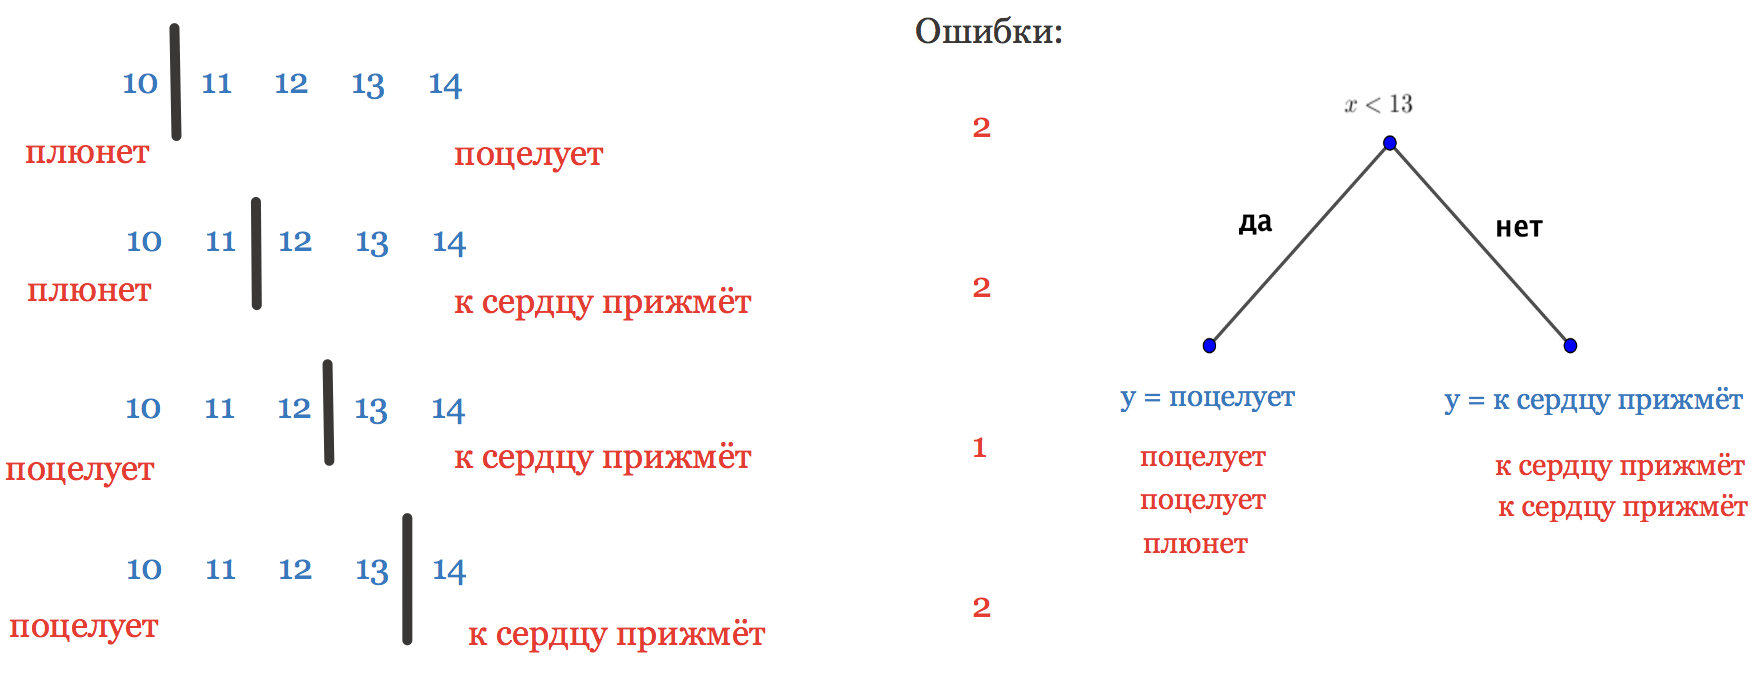
\includegraphics[scale=0.28]{class_tree_1.png}
	\end{center} 	
	
	Рассуждая аналогичном образом приходим к выводу, что самое классное разбиение между $12$ и $13$. При нём мы совершаем только одну ошибку.  В дереве, мы будем задавать вопрос: <<А количество лайков меньше $13$?>> Если да, будем идти налево и прогнозировать, что нас поцелуют. Если нет, будем идти направо и прогнозировать, что нас прижмут к сердцу. 
	
	Справа в листе дерева у нас оказались объекты одного класса. Слева в листе дерева содержутся объекты разных классов. Можно сделать ещё одно разбиение. 
	
	\begin{center}
		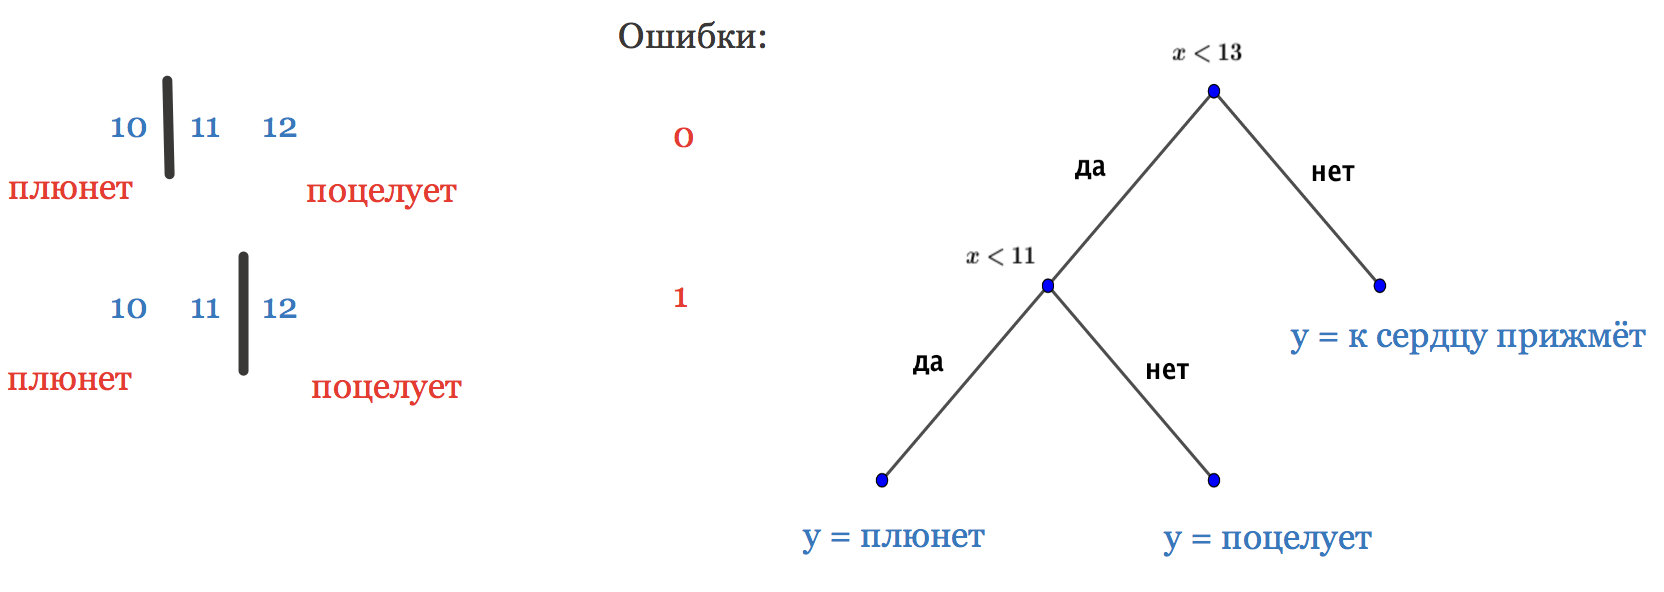
\includegraphics[scale=0.28]{class_tree_2.png}
	\end{center} 	
	
	В итоге в нашем дереве окажется три листа, в каждом из которых мы будем делать прогноз. Обратите внимание, что дерево запомнило выборку.  Деревья постоянно так делают. В этом их сушественный минус. Чтобы победить его, деревья стригут. Либо используют как части более сложных моделей. Например, как часть случайного леса. 
	
	Предположим, что под фоточками Маши от Паши накопилось $15$ лайков. Что ждёт её отношения? Начинаем идти по решающему дереву, чтобы сделать прогноз. Число лайков меньше $13$? Нет. Идём направо. Кажется, Машу прижмут к сердцу. Это наш прогноз.  	
}


\section*{Ещё задачи} 

Тут лежит ещё несколько задач для самостоятельного решения. Возможно, похожие будут в самостоятельной работе... 

\subsection*{Задача 6}

Пятачок собрал данные о визитах Винни-Пуха в гости к Кролику. Здесь $x_i$ - количество съеденного мёда в горшках, а $y_i$  - бинарная переменная, отражающая застревание Винни-Пуха при входе 

\begin{center}
	\begin{tabular}{c|c}
		$y_i$ & $x_i$ \\
		\hline
		0  & 1 \\
		1 & 4\\
		1 & 2\\
		0 & 3 \\
		1 & 3 \\
		0 & 1
	\end{tabular}
\end{center}

\begin{enumerate}
	\item[а)] Пятачок собирается оценить дерево по всей выборке.  Помогите очень маленькому существу сделать это. 
	\item[б)] Пятачок узнал у Иа-Иа, что оказывается выборку надо делить на тренировочную и тестовую Поэтому он отложил последние два наблюдения для теста. Оцените дерево по первым четырём наблюдениям и проверьте его работоспособность по последним двум. 	
\end{enumerate}

\ifbool{answers}{
	\textbf{Решение:}
	
	\begin{enumerate}
		\item[а)]  Бедный малютка Пяточок! Он даже не понимал, на какие муки он себя обрекает, когда собирался строить свою модель для прогнозирования того, что произойдёт с Винни! Как же хорошо, что мы оказались рядом и подставили маленькому существу своё большое дружеское плечо.  Для начала построим дерево сразу на всей выборке. 
		
		\begin{center}
			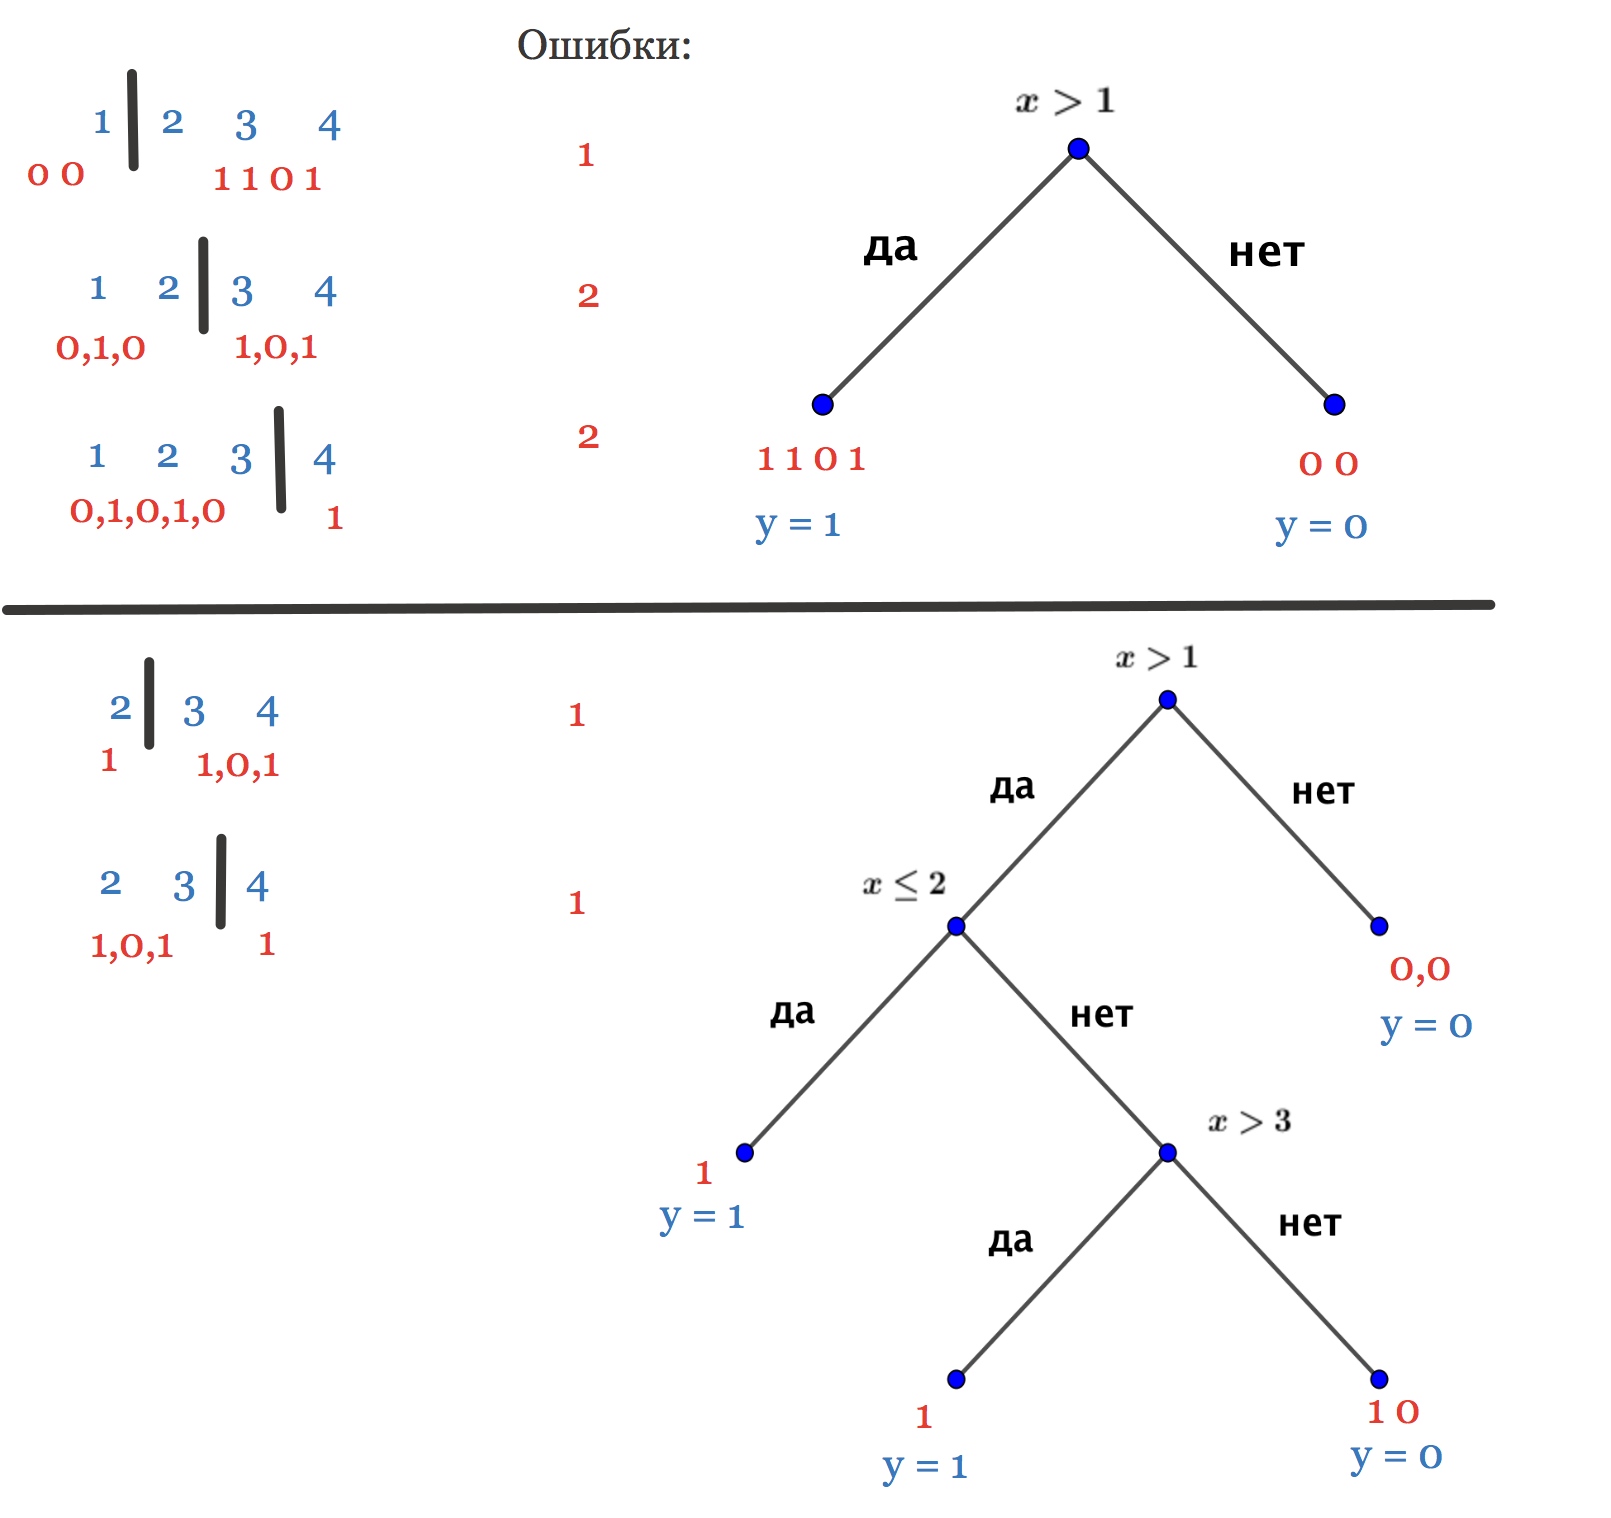
\includegraphics[scale=0.28]{class_tree_6.png}
		\end{center} 	
		
		Обратите внимание, что это дерево ошибается из-за того, что при  $x=3$ у нас есть как факт застревания медведя в норе, так и факт его прохождения сквозь нору. 
		
		\item[б)]  Когда мы строим дерево на первых четырёх наблюдениях, первое разбиение можно сделать либо по единице, либо по четвёрке. В обеих ситуациях совершается одна ошибка. Для удобства выберем первый случай. Дальше снова неважно где делать разбиение. Сделаем его в двойке. В итоге получим дерево из пункта а). На тестовой выборке дерево делает одну ошибку при $x=3$.
	\end{enumerate}
	
}

\subsection*{Задача 7}

Бандерлог начинает все определения со слов «это доля правильных ответов»:
\begin{enumerate}
	\item[а)] accuracy — это доля правильных ответов\ldots
	\item[б)] точность (precision) — это доля правильных ответов\ldots
	\item[в)] полнота (recall) — это доля правильных ответов\ldots
	\item[г)] TPR — это доля правильных ответов\ldots
\end{enumerate}

Закончите определения Бандерлога так, чтобы они были, хм, правильными.

\ifbool{answers}{
	\textbf{Решение:}
	
	\begin{enumerate}
		\item[а)] $\text{accuracy} = \frac{\text{TP} + \text{TN}}{\text{TP} +\text{FP} +\text{FN} +\text{TN}}$
		\item[б)] $\text{precision} = \frac{\text{TP}}{\text{TP} +\text{FP}}$
		\item[в)] $\text{recall} = \frac{\text{TP}}{\text{TP} +\text{FN}}$
		\item[г)] $\text{TPR} = \frac{\text{TP}}{\text{TP} +\text{FN}}$
	\end{enumerate}
}


\subsection*{Задача 8}

Бандерлог обучил модель для классификации и получил вектор предсказанных вероятностей принадлежностей к классу $1$. 

\begin{center}
	\begin{tabular}{c|c}
		$y_i$ & $b_i$ \\
		\hline
		$1$  & $0.9$ \\
		$0$ & $0.1$ \\
		$0$ & $0.75$ \\
		$1$ & $0.56$ \\
		$1$ & $0.2$ \\
		$0$ & $0.37$ \\
		$0$ & $0.25$ \\		
	\end{tabular}
\end{center}

\begin{enumerate}
	\item[а)]  Бинаризуйте ответ по порогу $t$ и посчитайте точность и полноту для $t = 0.3$ и для  $t = 0.8$.
	\item[б)]  Какой порог бы вы выбрали? 
	\item[в)]  Постройте ROC-кривую и найдите площадь под ней. 
\end{enumerate}


\ifbool{answers}{
	\textbf{Решение:}
	
	\begin{enumerate}
		\item[а)]  Построим в нашей табличке две колонки с прогнозами. Для удобства. 
		
		\begin{center}
			\begin{tabular}{c|c|c|c}
				$y_i$ & $b_i$ & $t=0.3$  & $t=0.8$\\
				\hline
				$1$  & $0.9$ & $1$ & $1$ \\
				$0$ & $0.1$ & $0$ & $0$\\
				$0$ & $0.75$ & $1$ & $0$\\
				$1$ & $0.56$ & $1$ & $0$\\
				$1$ & $0.2$ & $0$ & $0$ \\
				$0$ & $0.37$ & $1$ & $0$\\
				$0$ & $0.25$ & $0$ & $0$ \\		
			\end{tabular}
		\end{center}
		
		Построим для обоих порогов матрицы ошибок. Слева матрица, соответствующая порогу $0.3$, справа матрица, соответствующая порогу $0.8$.
		
		\begin{minipage}[t]{0.45\textwidth}
			\begin{tabular}{|c|c|c|}
				\hline
				& $y=1$  &  $ y = 0$ \\  \hline 
				$\hat y = 1$  &   $2$ &    $2$ \\      \hline 
				$\hat y = 0$ &   $1$ &    $2$ \\      \hline 
			\end{tabular}
		\end{minipage}
		\begin{minipage}[t]{0.45\textwidth}
			\begin{tabular}{|c|c|c|}
				\hline
				& $y=1$  &  $ y = 0$ \\  \hline 
				$\hat y = 1$  &   $1$ &    $1$ \\      \hline 
				$\hat y = 0$ &   $2$ &    $3$ \\      \hline 
			\end{tabular}
		\end{minipage}
		
		Считаем для обоих случаев точность и полноту. 
		
		\begin{equation} 
		\begin{aligned}
		&Precision_1 = 0.5     \qquad &Recall_1 = 0.66  \\ 
		&Precision_2 = 0.5  \qquad &Recall_2 =  0.33   \\ 
		\end{aligned}
		\end{equation} 
		
		\item[б)]  Обе модели дают одинаковую точность при разной полноте. У первой модели полнота повыше, имеет смысл выбрать её (но это неточно, надо бы это проверить на большем числе данных). 
		
		\item[в)] Построим roc-кривую. Для этого отсортируем все наблюдения в нашей табличке по возрастанию.
		
		\begin{center}
			\begin{tabular}{c|c}
				$y_i$ & $b_i$ \\
				\hline
				$1$  & $0.9$ \\
				$0$ & $0.75$ \\
				$1$ & $0.56$ \\
				$0$ & $0.37$ \\	
				$0$ & $0.25$ \\			
				$1$ & $0.2$ \\												
				$0$ & $0.1$ \\
			\end{tabular}
		\end{center}
		
		Заведём сетку размера 4 на 3 и начнём делать шаги по ней так, как было описано во второй задаче.
		
		\begin{center}
			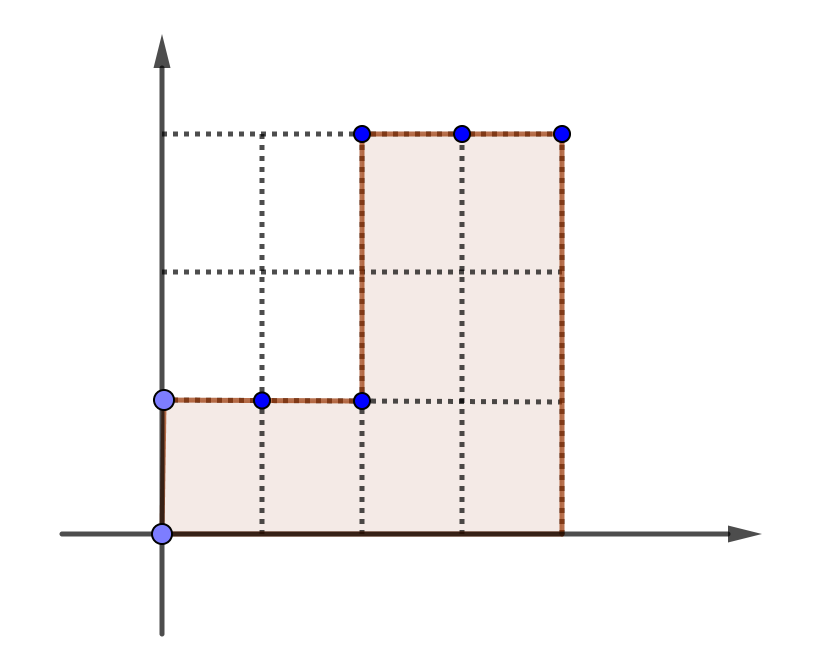
\includegraphics[width=.4\paperwidth]{roc_auc2.png}
		\end{center}
		
		Профит, получили roc-кривую.  Видим, что площадь под ней равна $\frac{8}{12}$. Иным языком говоря, среди $12$ пар ноликов и единичек, вероятности отсортированы так, как нам хотелось бы $8$ раз. 
		
		Для первого наблюдения $(1, 0.9)$ все четыре пары верны. Для второго $(1, 0.56)$ будет одна ошибочная сортировка, для третьей $(1,0.2)$ будет три ошибочных сортировки. 
	\end{enumerate}
	
}


\end{document}
